\documentclass[withoutpreface,bwprint]{cumcmthesis} %去掉封面与编号页
\usepackage[framemethod=TikZ]{mdframed}
\usepackage{url}   % 网页链接
\usepackage{subcaption} % 子标题、
\usepackage{graphicx}
\title{“信息引航者”——基于MGCA的信息推荐系统}
\usepackage{listings}
\lstset{language=Matlab}
\usepackage{pythonhighlight}
\usepackage{setspace}
\begin{document}
	
	\maketitle\thispagestyle{empty}
	\begin{abstract}
		随着互联网上信息的越来越多,想要在海量信息中获取我们感兴趣或有需求的信息愈加困难。推荐系统的出现正是为了解决这种\textbf{“信息过载”}的问题。推荐系统已在互联网中得到了广泛的应用,并给应用它的企业带来了\textbf{丰厚的利润}。有关推荐系统的研究具有十分深远的意义与巨大的实用价值,我们的项目\textbf{《 “ 信息引航者”——基于MGCA的信息推荐系统》 }就是为了解决“信息过载”问题,响应国家发展和改革委员会“新基建”号召,创造巨大经济价值而设计的一款推荐系统,并在此基础上进行了商业构想,制定了完整的商业计划。\par
		技术路线上,我们设计了一种\textbf{考虑多种粒度信息的候选感知推荐算法},并在微软发布的MIND数据集上进行新闻推荐任务,通过\textbf{知识图谱、图神经网络、Transformer、Fastformer}等基础模型组成\textbf{MGCA( Multi-grained Candidate-aware)模型},聚合不同粒度的候选感知信息与候选新闻匹配推荐用户兴趣咨询信息,在微软的MIND数据集Small版本新闻推荐任务成为\textbf{SOTA模型},暂时为该数据集上新闻推荐任务AUC、MRR、nDCG等指标\textbf{最高的模型},比2022年清华大学Tao Qi等人提出的SOTA模型KIM的AUC、MRR、nDCG@5,nDCG@10指标分别高\textbf{1.00、1.33、0.63、0.96}个百分点。\par
		商业计划上,我们制定了完整的创新商业构建。产品营销定位\textbf{全国由于算法、算力壁垒急需但难求个性化推荐系统的中、小企业},致力于助力中、小企业拥有自己的个性化推荐系统,促进推荐系统的广告、增值服务、电商、节省成本变现。盈利方式聚焦B端企业,提供\textbf{低耦合工业界解决方案或完整软件系统},适应不同类型企业的不同需求。财务管理单设财务部进行,其中软件成本计算采取Barry Boehm提出的\textbf{COCOMO模型}。市场竞争分析按照\textbf{SWOT模型}进行分析,充分考虑团队优势劣势。营销方式上,根据Raymond Vemon教授的\textbf{产品生命周期理论},按照团队发展的不同阶段采取不同的营销模式。营销策略上不同于传统的“7P+4C”策略,我们采取\textbf{“六位一体”的扁平化多层化营销策略}。\par
		工程落地上,我们在\textbf{Python3.6和Tensorflow1.15}框架的环境下进行算法的研发设计与实验研究,在\textbf{JAVA jdk1.8}的环境下,前端采取\textbf{Vue3、Bootstrap}框架,后端采取\textbf{SpringBoot}框架进行软件开发。在完整软件开发的流程中,采取\textbf{原型软件生命周期模型}组织开发,不断适应复杂多变的需求,提高B端企业客户体验,为了规避原型模型难以规划和管理的弊端,\textbf{定期核验开发进展},进行\textbf{兼容性测试与稳定性测试},确保项目正常运行。\par
		\textbf	{关键字: MGCA( Multi-grained Candidate-aware)模型\quad  COCOMO模型\quad  SWOT\quad  “六位一体”扁平多层化营销策略\quad   Tensorflow\quad SpringBoot\quad  原型软件生命周期模型\quad	}
	\end{abstract}
	\setcounter{page}{1}
	\tableofcontents
	\newpage
	\section{引言}
	\subsection{研究背景及意义}
	\subsubsection{ 信息过载问题的解决迫在眉睫} 
	互联网高速发展,信息呈爆炸式增长,用户逐渐由信息匮乏时代迈入了信息过载时代——过量信息反而使得用户无法找到自己需要的信息。信息过载问题会产生一系列问题,比如用户体验变差、用户数量骤减、用户粘性降低等。
	信息爆炸的今天,个性化新闻推荐技术已经变成了许多新闻网站和App的关键技术。新闻的数据来源众多,可能一分钟就有成千上万条新的数据产生,在数据量激增的情况下,需要付出更多的人力成本,并且人工处理速度慢,效率十分低下。一套个性化新闻推荐系统刚好可以应用于有效缓解这种信息过载问题。如图1是新闻推荐系统通过个性化推荐实现精准化投放信息的流程示意。
	\begin{figure}[H]
		\centering
		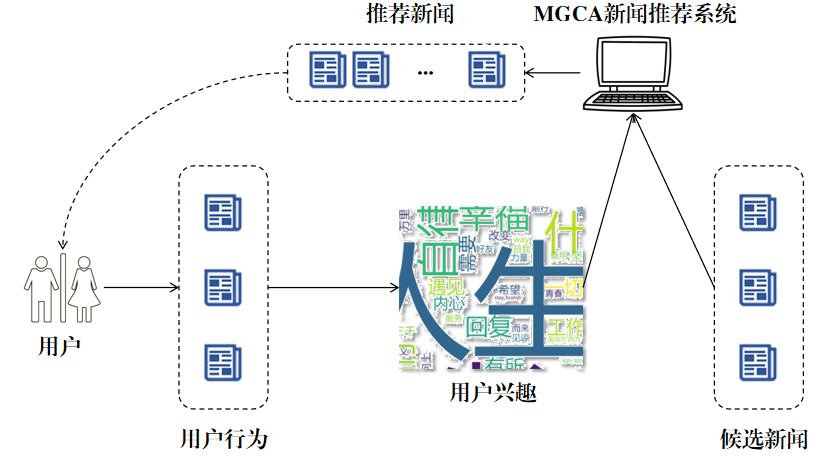
\includegraphics[width=0.95\textwidth]{2}
		\caption{个性化新闻推荐系统实现精准化投放信息}
		\label{fig:circuit-diagcam}
	\end{figure}
	\subsubsection{ 互联网与推荐系统的融合带来巨大的经济价值}
	目前互联网变现的主要方式均可以与推荐系统融合起来,创造巨大的经济价值,如图2展示了推荐系统与互联网融合时创造价值的几种常见途径:
	\begin{figure}[H]
		\centering
		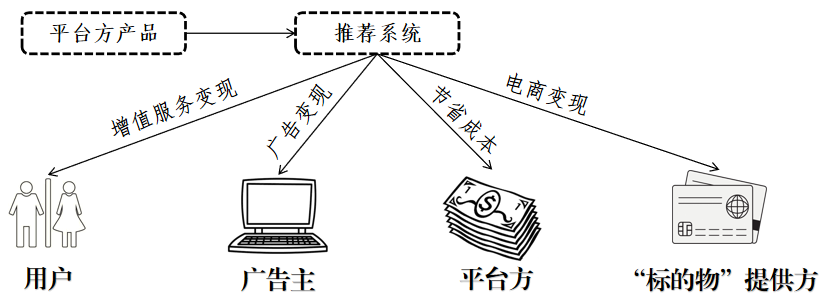
\includegraphics[width=0.95\textwidth]{1}
		\caption{推荐系统与互联网融合体现的经济价值}
		\label{fig:circuit-diagcam}
	\end{figure}
	$\bigstar$\textbf{广告变现:}用户方产品在互联网上投放广告,通过提高广告曝光以及用户点击广告获取权益。通过推荐系统的应用,可以在新闻APP中实现广告精准投放。广告业务偏轻公司一般都会选择流量外包方式做广告变现,\textbf{通过推荐系统提高广告精准投放率与用户点击率即是一种非常好的方式。}\par
	$\bigstar$\textbf{增值服务变现:}增值服务主要是指基本服务以外的特色服务,如新闻平台常见的会员制。推荐系统通过精准把握用户兴趣,引导用户购买会员增值服务产品。推荐系统的个性化推荐服务不仅可以更加深层次的挖掘用户需求,还可以使更多相对冷门但优质的内容得到曝光与展示。在 2004 年,一位杂志主编在形容亚马逊和 Netflix 的商业模式时首次提出“长尾”概念,指代需求和销量不高的产品在市场中所占比例与主流产品相当甚至更高。当传统的二八定律无法再创造更多利润时,商家开始关注“长尾”潜在的商业价值,即专注于小众群体的个性化偏好。\textbf{推荐算法在实现企业从二八定律向“长尾效应”转变方面发挥着重要作用。}以往市场只关注大众需求,而通过推荐系统,个性化需求也可以得到满足,提高了用户的满意程度和消费质量,实现了双赢。\par
	$\bigstar$\textbf{节省成本变现:}在推荐算法还不作为推荐系统的重要组成部分之前,推荐这项工作的大部分还是由人工完成的,根据一些专业人士的建议和想法,来向用户推荐产品及服务。推荐系统对平台方的贡献不仅在于直接的商业价值或是促进用户粘性、用户数量增长等,还可以\textbf{用更少的成本实现最大程度的个性化新闻推荐,提高内容的分发效率。}\par
	$\bigstar$\textbf{电商变现:}无论是传统意义的实体电商产品,还是网络小说、网络课程等虚拟电商产品,都可以通过提高分发商品效率,精准化投放促进商品售卖而提高商家分成,吸引商家入驻。总的来说,\textbf{在电商变现方面,推荐系统可以做到促进“标的物”提供方的生态逐步健全繁荣,获取更多经济效益。}\par
	\subsubsection{ 响应国家发展和改革委员会“新基建”号召}
	国家发改委于2020年4月首次明确了新型基础设施的范围包括以人工智能、云计算、区块链等为代表的新技术基础设施,新型基础设施建设对于打造经济新动能、重塑供应新链条、促进惠民新模式有重大意义,是当前稳经济、促增长的核心支撑。人工智能、云计算、物联网等现代信息科技依托新型基础设施建设得到了高速发展。\par
	特别是处于疫情后时代,线下娱乐受到重创,线上娱乐成为青年群体最重要的娱乐方式之一。在当前的时代背景下,推荐系统的研究有助于\textbf{促进青年群体的幸福感,扩大新型基础设施建设的有效投资,有效对冲经济下行压力,有力支撑经济社会高质量恢复与持续发展。}
	\subsection{相关研究现状}
	推荐系统是学术界和工业界研究的热门话题。学术界侧重理论层面的分析和模型性能的提升,而工业界更侧重实践层面的发展以及用户体验的提升以及推荐系统的应用前景。下面从这两方面分别介绍。
	\subsubsection{ 推荐系统在工业界的应用与发展前景}
	在移动互联网快速发展、智能手机普及以及信息产生爆炸增长的背景下,高效获取对个人有价值的信息变得愈发重要。推荐系统作为一种高效的信息过滤工具,在用户精准高效获取信息方面起到了重要作用。它不仅解决了用户需求不明确时的信息获取问题,也在内容分发、用户体验和商业变现方面发挥着关键作用。推荐系统已经成为toC互联网产品的标配技术,并给应用它的企业带来了丰厚的利润。据报道,推荐系统给亚马逊带来了35\%的销售收入,给Netflix带来了高达75\%的消费,并且Youtube主页上60\%的浏览来自推荐服务。如下表1所示,常见的推荐系统以及推荐内容与使用的特征表,展示了国内应用了推荐系统的常见应用。\par
	\begin{table}[H]
		\centering
		\caption{不同推荐场景下的推荐内容和特征}
		\begin{tabular}{|m{2cm}|m{4cm}|m{4cm}|m{4cm}|}
			\hline
			推荐场景 & 推荐产品 & 推荐项 & 推荐使用的特征 \\
			\hline
			资讯推荐 & 今日头条、百度新闻、腾讯新闻、知乎 & 新闻标题、内容、主题 & 用户行为、用户画像、年龄、性别、教育背景 \\
			\hline
			快资讯 & 抖音、快手、西瓜视频、YouTube & 视频内容、音频、类型 & 热度、标题和描述、用户行为 \\
			\hline
			腾讯视频 & 爱奇艺、优酷、HBO、Netflix & QQ音乐、网易云音乐 & 音频类型、演唱者、作曲者等 \\
			\hline
			电商推荐 & 淘宝、京东、亚马逊、拼多多 & 商品 & 商品标题、描述、图片、类别、流行度 \\
			\hline
		\end{tabular}
	\end{table}
	推荐系统的发展与大环境和技术进步密不可分,接下来我们从三个层面分析推荐系统发展的前景:\par
	$\bigstar$\textbf{政策层面:}在当前“智能化”的时代背景下,国家空前把人工智能提升到了战略的高度,政策的大力支持、媒体的大肆宣扬以及样板示范作用,让个性化新闻推荐的产品与业务受到了更多投资人、专家的重视,这不仅极大推动了新闻推荐系统的发展,也有利于推荐系统在更多的业务场景下落地。\par
	$\bigstar$\textbf{教育层面:}国内从2016年起步开始开设数据科学与大数据技术、智能科学与技术等人工智能相关专业,推荐系统作为大数据和人工智能领域业务价值最大之一的领域,极大的受益于大数据与人工智能相关学科人才的增长,这为助力推荐系统进一步发展提供了基础。\par
	$\bigstar$\textbf{科技层面:}构建一套灵活实时、准确度高、稳定高效的新闻推荐系统是非常困难的,它不仅涉及到业务场景,还与产品交互、工程应用密不可分,几乎只有中、大规模的公司才会构建一套推荐算法业务体系,但受益于云计算基础设施的逐步健全,创业公司可以利用云平台提供的SAAS服务搭建自己的推荐系统模块,降低了推荐系统的使用门槛,促进了推荐系统更加广泛的应用。\par
	\subsubsection{ 推荐系统在学术界的研究现状}
	根据用户日志的数据的输入形式和推荐算法的设计机制,推荐系统在学术界的发展主要包含以下三个阶段:基于协同过滤的推荐、基于内容的推荐以及混合推荐。\par
	$\bullet$\textbf{基于协同过滤的推荐:}协同过滤推荐算法是诞生最早且比较著名的推荐算法,这种算法主要考虑了用户与与用户之间的相似度,在所有用户群体中找到与用户具有相似兴趣、相似偏好的的用户感兴趣的产品或服务推荐给用户。例如下图3中的情景,小林喜欢《间谍过家家》和《干物妹小埋》这类喜剧动漫片,小浩也喜欢看喜剧动漫,如《间谍过家家》、《干物妹小埋》和《工作细胞》等。基于相似喜好,在协同过滤算法中会将小林未看过但小浩喜欢的动漫《工作细胞》推荐给小林。\par
	\begin{figure}[H]
		\centering
		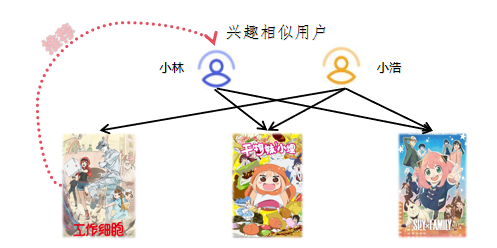
\includegraphics[width=0.65\textwidth]{3}
		\caption{协同过滤推荐示例}
		\label{fig:circuit-diagcam}
	\end{figure}
	目前学术界已提出多种协同过滤的推荐算法,包括传统的矩阵分解方法和结合深度学习技术的新型方法。传统方法存在冷启动和数据稀疏等问题,而深度学习结合的方法如Autoencoders、CDAE和DMF能更好地解决这些问题,通过学习用户和项的潜在因子来提高推荐性能。尽管协同过滤在工业界得到广泛应用,但仍面临冷启动等挑战,需要进一步研究完善。\par
	$\bullet$\textbf{基于内容的推荐:}这种算法不同于协同过滤算法,根据用户的交互记录为用户提供个性化推荐结果,基于内容的推荐算法的基本原理是根据用户和项的属性特征以及用户的历史行为,获得用户的兴趣偏好,为用户推荐跟他的兴趣偏好相匹配的项。例如小琰经常浏览与各地旅游攻略相关的资讯,基于内容的推荐算法则可能推荐近期爆火的旅游地相关新闻。\par
	基于内容的推荐方法早期采用统计策略,如TF-IDF和余弦相似度,存在内容相同但物品不同的问题。后续方法利用机器学习技术如决策树、最近邻居和神经网络解决这一问题,比如DeepWide和DeepFM。目前主流的基于深度神经网络的推荐算法使用CNN、RNN、注意力网络或记忆网络从用户历史交互序列中提取特征,例如DeepJoNN、ATEM和MANN。为克服错误关系假设,一些方法利用神经网络挖掘用户的长期兴趣和短期兴趣,融合长短期兴趣做个性化推荐,这称为以会话为主的推荐方法。\par
	$\bullet$\textbf{混合推荐:}混合推荐算法进一步提升了推荐系统的性能,融合了知识图谱的信息,增加了推荐系统内部算法的可解释性。利用知识表示学习技术将丰富语义信息融入推荐过程,使结果更准确满足用户需求。混合推荐方法建立用户知识图谱,利用路径推理、强化学习和图神经网络技术将购买关系建模为知识图谱的补全任务,从中学习用户和项的表示并预测匹配概率,即向用户推荐该项的概率。比如较为经典的 KPRN 方法使用循环神经网络挖掘用户与物品之间的图谱路径,利用知识图谱的路径推理技术建模用户与候选推荐项的可解释性推荐。这一前沿技术解决了推荐算法黑盒问题,提高了推荐结果的可解释性,是未来推荐系统的重要研究方向。\par
	表 2 列举了上述三类方法的经典模型、各模型使用的核心技术以及评测指标等。
	\begin{table}[H]
	\centering
	\caption{三类方法的核心技术对比}
	\begin{tabular}{|m{2cm}|m{4cm}|m{4cm}|m{4cm}|}
		\hline
		推荐场景 & 方法举例 & 核心技术 & 评价指标 \\
		\hline
		协同过滤推荐方法 & Autoencoders、CADE、DMF、CKE & 矩阵分解、张量分解、神经网络 & accuracy、MRR、ndcg@k \\
		\hline
		基于文本内容推荐 & TransRec、DeepCoNN、JRL、DKN、DAN & 卷积神经网络、循环神经网络、注意力机制 & accuracy、MRR、ndcg@k \\
		\hline
		混合推荐方法 & KPRN、RippleNet、KGCN、VGAE、PGPR & 强化学习、图卷积神经网络、深度神经网络、注意力神经网络 & accuracy、MRR、ndcg@k \\
		\hline
	\end{tabular}
	\end{table}
	\subsection{项目架构总览}
	\subsubsection{ 项目整体框架}
	本项目的整体框架主要包含营销策略、模型框架、工程落地三个阶段,结合了实际应用和技术发展趋势,就创新业务做商业计划分析和原型搭建,实现了IT与业务的相对齐。\par
	\begin{figure}[H]
		%\centering
		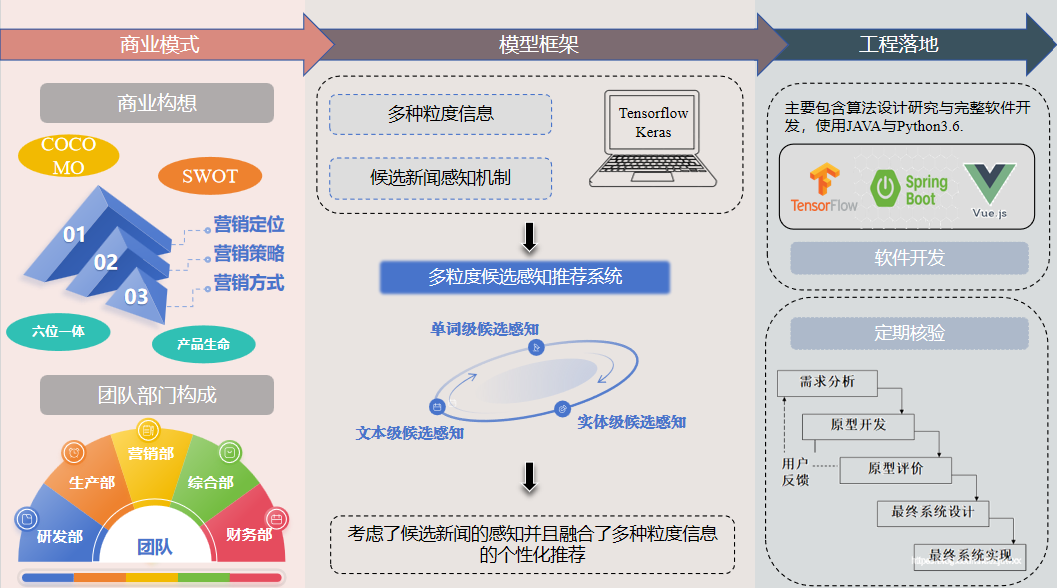
\includegraphics[width=1.0\textwidth]{框架}
		\caption{项目框架图}
		\label{fig:circuit-diagcam}
	\end{figure}
		$\bigstar$\textbf{模型框架:}基于之前的研究,我们提出了一种融合多种粒度信息的候选感知推荐系统,并在微软的公开数据集MIND数据集上进行新闻推荐任务上得到了截止目前AUC、MRR、nDCG@5,nDCG@10等指标最高的模型,在transformer头数、fastformer头数、学习率、优化器等参数确定情况下,比2022年清华大学Tao Qi等人在Personalized News Recommendation with Knowledge-aware Interactive Matching中提出的SOTA模型KIM的AUC、MRR、nDCG@5,nDCG@10指标分别高\textbf{1.00、1.33、0.63、0.96}个百分点,是该数据集的Small版本当前国内AUC、MRR、nDCG@5,nDCG@10指标最高的模型。\par
		模型的算法框架主要包含两个部分:多粒度用户点击新闻编码器、候选新闻编码器。多粒度用户点击新闻编码器主要包含单词级、新闻级、实体级三种粒度的信息,可以充分挖掘用户点击的信息在不同粒度信息的潜在内容,更加细致的挖掘用户兴趣,其中实体级粒度编码器与候选新闻编码器中的实体信息是与用户点击新闻通过知识编码器交互式学习得到。在候选新闻编码器中,候选新闻通过新闻编码器得到的信息与知识编码器中得到的信息聚合后再次通过Transoformer、Fastformer聚合到用户点击新闻中,最终聚合三个粒度的信息与候选新闻编码器得到了候选新闻信息进行匹配得到匹配分数,进行个性化新闻推荐。这样的推荐不仅感知了候选新闻与用户历史点击新闻的关联信息,还考虑了不同粒度信息中不同的潜在推荐价值,相比以往模型具有显著优越性。如下图5所示,算法框架的整体结构图。\par
		\begin{figure}[H]
			%\centering
				\includegraphics[width=1.0\textwidth]{MGCA}
			\caption{算法架构图}
			\label{fig:circuit-diagcam}
		\end{figure}
	    $\bigstar$\textbf{商业计划:}本产品营销定位全国由于算法、算力壁垒急需但难求个性化推荐系统的中、小企业,致力于助力中、小企业拥有自己的个性化推荐系统,促进推荐系统的多元化变现,提高广告的转化率与曝光、促进“标的物”提供商家的生态繁荣、促进“标的物”售卖。ToB,指公司的产品或服务所面向的用户是企业,围绕企业的生产、管理、运营、决策等环节制定相应的产品服务,团队盈利方式\textbf{聚焦toB端},主要包含\textbf{提供整套低耦合工业界解决方案和成熟的整套解决方案}。低耦合工业界解决方案通过提供近零耦合的代码段供企业直接聚合到自己推荐系统中创造价值。同时在我们的商业计划构想中,团队包含专业的软件开发人员,可以直接为不具备软件开发能力的企业直接提供成熟的整套软件,满足企业的个性化需求,并且将我们的推荐系统嵌入其中。团队会建立商业量化指标体系,保证推荐系统真正的落地业务。\par
	    团队成立初,共包含研发部、生产部、营销部、综合部、财务部等部门。团队成立初产品类型有限,但软件开发需求复杂多变,团队成立生产部用于进行软件开发活动。设立财务部单独管理财务,其中,软件开发的成本估算采用Barry Boehm在1981年提出的\textbf{COCOMO模型}计算,这是一种基于代码行的回归模型,考虑了软件项目开发过程中的大小、工作量、成本、时间、质量。
	    在市场竞争分析中,我们使用\textbf{SWOT模型}进行分析( Strengths,Weakness,Opportunesses,Treats),充分考虑了团队的优势、劣势、机会和威胁风险之间的关系。
	    在营销模式中,根据Raymond Vemon教授的产品生命周期理论,我们按照团队发展的三个阶段( 前期、中期、后期)制定了不同的营销模式。不同于传统的“7P+4C”营销策略,我们采取\textbf{“六位一体”式的扁平化多层化式营销方式}。\par
	    $\bigstar$\textbf{工程落地:}在算法的研发和设计阶段在\textbf{Python3.6的Tensorflow框架}下进行,使用VSCode、Pycharm等工具进行编码实现与实验研究。在完整的软件方案开发过程中,我们主要使用JAVA在jdk1.8环境下进行,前端框架主要采取\textbf{Vue3,bootstrap},后端框架主要采取\textbf{SpringBoot},开发平台选用IDEA。在软件开发的周期中,为了应对模糊不清、复杂多变的需求,我们采取\textbf{原型模型}的思想组织软件开发人员进行开发,在开发过程中不断适应需求、增进对需求的理解,对于B端企业客户也是学习使用软件的过程,便于确定系统的性能、服务的质量、设计的可行性,同时,为了规避原型软件周期模型难以规划和管理的缺点,团队将组织定期\textbf{核验开发进展},确保开发顺利进行。在软件开发过程中,我们严格按照软件开发流程进行\textbf{数据库E-R图设计、UML设计},并在每次的核验中进行兼容性与稳定性测试,确保项目正常运行。\par
	\subsubsection{ 项目优势与创新性}
	$\bigstar$\textbf{算法考虑了多种粒度信息的候选新闻感知,适应用户不同粒度的行为信息:}以往的模型有些虽然考虑了用户点击新闻与候选新闻的关联信息,但它们仅仅只是将候选新闻与用户的兴趣进行建模,没有将其融合到多种粒度的信息中考虑,我们的模型考虑多种粒度信息的候选新闻感知,在微软的MIND数据集Small版本上成为当前任务的\textbf{SOTA模型},暂时在AUC、MRR、nDCG等指标\textbf{领先国内},下面的例子可以很好的具象化我们模型的优越性:如图6所示,第一个点击的新闻包含了“拼多多”、“买家秀”,这些词与第一个候选新闻的“拼多多”有关。第二个点击新闻也与第一个候选新闻有单词级的关联,因为它们都包含同一个单词“拼多多”。基于单词级的相关性可以推断用户可能对第一个候选新闻感兴趣。使用知识图谱进行点击新闻和候选新闻之间的实体匹配,有助于更好地理解用户对候选新闻的兴趣。例如,第三个点击新闻中的实体“《 黑铁的鱼影》” 与第二个候选新闻中的实体“《 名侦探柯南》” 具有固有的相关性。《黑铁的鱼影》是《名侦探柯南》 的剧场版影视,通过知识图谱根据实体级匹配可以推断出用户可能对第二个候选新闻感兴趣。因此,利用不同粒度信息之间的相关性有利于兴趣匹配。\par
	\begin{figure}[H]
		\centering
		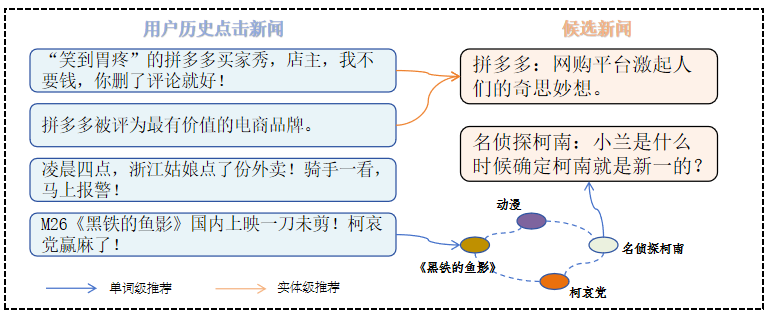
\includegraphics[width=0.9\textwidth]{sample}
		\caption{体现不同粒度信息对于新闻推荐重要性的一个例子}
		\label{fig:circuit-diagcam}
	\end{figure}
	$\bigstar$\textbf{商业计划完善,可以适应市场变化:}我们的市场定位非常清晰——聚焦B端企业。我们制定了完善的商业计划,包含了完整的团队构成、财务计算方法、市场竞争分析和营销策略方法。团队构成上研发部、生产部、营销部、综合部、财务部各司其责,完成算法改进、软件开发、宣传营销、协助协调。财务管理等各自要务,并且保持交流沟通。财务计算方法上创新性的采用了COCOMO模型计算软件开发成本,按照基础、中级、细致三个模型阶段分别计算,精确掌握开发成本,合理定价,适应市场变化。\par
	在营销策略中创新性的采取“六位一体”的扁平化多层化营销策略,如下图7,我们按照团队发展的前期、中期、后期三个阶段,分别制定了不同的营销模式,主要包含前期营销模式( 互联网云平台营销、线下开放式营销、服务体验与客户开发式营销)、中期营销模式( 中间商代理营销、专家营销)和后期营销模式( “ 一对一”互动制定化营销、品牌营销)。在互联网时代,三个时期的营销模式中我们都与互联网紧密结合,试图碰撞出更大的火花。\par
	\begin{figure}[H]
		%\centering
		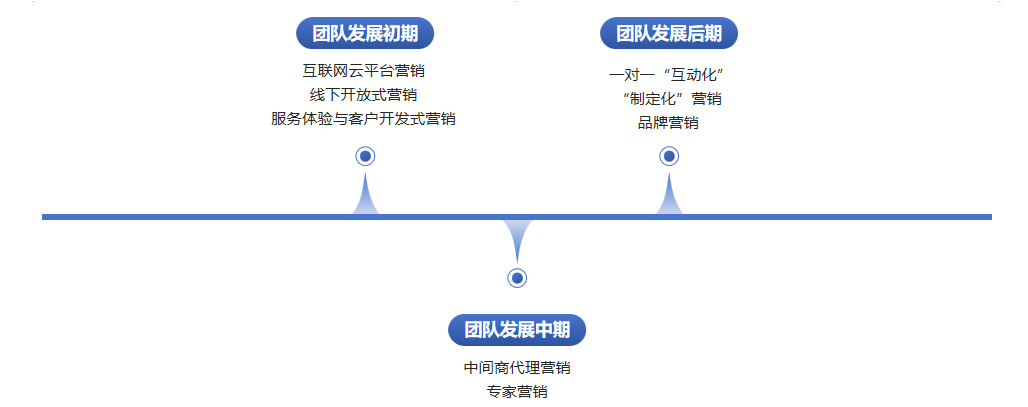
\includegraphics[width=0.95\textwidth]{营销发展}
		\caption{团队发展的不同时期采取不同的营销模式}
		\label{fig:circuit-diagcam}
	\end{figure}
	$\bigstar$\textbf{软件开发流程专业,适应B端企业的个性化需求:}团队人员具备专业的软件开发能力,为B端企业提供两种方案——低耦合工业界解决方案和成熟软件系统,以适应不同企业的需求。在下文中我们给出了一个完整的软件项目落地示例,软件生命周期采取了原型化模型的思想,不断地具象化最终的完整软件,在此过程中方便B端企业客户不断适应软件的使用,并且及时修改,满足企业端客户的个性化需求。此外,我们通过定时核验的兼容性测试与稳定性测试规避了原型模型难以规划和管理的缺点。\par
	\newpage
	\section{模型技术路线及实现方案}
	\subsection{数据集选取}
	\subsubsection{ MIND数据集}
	MIND是微软在2020年发布的公开数据集(https://msnews.github.io/index.html),其包含了2230000条用户行为记录。MIND是目前新闻推荐算法研究领域应用最广泛的大规模数据集,主要包含behaviors.tsv和news.tsv这2个文件。behaviors.tsv收集了微软新闻平台下匿名用户的行为日志,news.tsv为新闻文章的文本信息。MIND数据集有2个版本:MIND-small和MIND-large。本项目所有研究采用MIND-small数据集,MIND-small数据集是在MIND上随机抽取的50000条记录,并且已经被划分为训练集和测试集。MIND-small中的每条用户行为记录包含了用户ID,用户点击过的新闻等信息。对于用户行为中涉及的所有新闻,MIND-small还提供了新闻对应的类别、标题、摘要、下载链接和实体等信息。
	\subsubsection{ glove词嵌入}
	我们采用Tensorflow用于模型实现,在我们的实验中,词嵌入是300维的,并且由glove词嵌入初始化。实验中只使用了新闻标题中的前30个单词和新闻中的前5个实体。从知识图中为每个实体选择10个邻居。实体嵌入是通过TransE从维基数据中提取的知识元组上的100维向量预训练。
	\subsection{方法介绍}
	\subsubsection{ 图神经网络}
	与传统的神经网络采用网格状数据进行建模不同,图神经网络(GNN)可以采用图顶点展现更复杂的建模能力。图主要是由多个节点v和边E构成的,$\mathbf{G=(v,E)}$,设图G中某个顶点v所包含的特征状态为
	\begin{equation}
		\mathbf{h_v} = f(\mathbf{x_v},\mathbf{x_E},\mathbf{h}_v\textsuperscript{'},\mathbf{x}_v\textsuperscript{'})
	\end{equation}
	其中,$h_v$为v的特征状态;$x_v$为v的特征因子;$x_E$为连接边的特征因子; $\mathbf{h}_v\textsuperscript{'}$ 和 $\mathbf{x}_v\textsuperscript{'}$ 分别为v的相邻顶点
	的状态输入和特征向量;f为过渡函数。
	
	根据顶点v的 $h_v$ 和 $x_v$ 值,将两者传输至输出函数g,得到顶点v的输出 $\mathbf{o_{v}}$,
	\begin{equation}
		\mathbf{o_v} = g(\mathbf{h_v,x_v})
	\end{equation}
	
	设H和X分别表示图顶点的特征状态堆叠及特征因子堆叠,则经过全局过渡函数运算之后,即t+1轮迭代后,对每个顶点进行损失求解,得到总 GNN 的总损失值,计算方法为:
	\begin{equation}
		\mathbf{loss} = \mathbf{\sum_{v=1}^{p} t_v - o_v }
	\end{equation}
	式中:p为顶点总数;$t_v$为顶点v的实际值。
	\subsubsection{ 注意力机制}
	自注意力机制适用于处理序列数据。通过自注意力机制,模型能够根据输入序列中不同位置的相关性动态地学习每个位置的表示,并将这些表示结合起来以形成最终的序列表示。这种机制使得模型能够捕获长距离依赖关系,避免了传统循环神经网络(RNN)中存在的梯度消失或爆炸问题。通过这种方式,自注意力机制提高了模型对全局上下文的理解能力,提升了模型在各种自然语言处理任务中的表现。在Transformer等基于注意力机制的模型中,自注意力机制被广泛应用,并取得了在机器翻译、文本生成等任务中的显著成果,成为当前深度学习领域中备受关注的技术之一。
	通过引入注意力机制,我们的模型能够以更加灵活的方式对输入序列进行建模,并且能够动态地调整对不同部分的关注程度。这一点对于处理长序列数据尤为重要,因为传统的固定权重机制往往无法有效捕捉到序列中不同部分之间的复杂关联。我们按照以下公式计算注意力权重:
	\begin{equation}
		\mathbf{u}_w = \text{softmax}(\mathbf{W} \cdot \hat{G}^T + \mathbf{b}) \cdot \hat{G} 
	\end{equation}
	其中,$\hat{G}$ 表示用户兴趣的表示,$\mathbf{W}$ 和 $\mathbf{b}$ 是模型参数。这个公式的核心是通过对用户兴趣表示进行加权求和,从而得到最终的用户兴趣表示。这种动态的注意力权重计算方式使得模型能够更加准确地捕捉到用户兴趣的细微变化,从而提高了模型的表达能力和泛化能力。
	\subsubsection{ Transformer }
	Transformer是一种基于自注意力机制的神经网络,与传统的 RNN 和 CNN 不同,Transformer  网络没有循环和卷积结构,因此能够并行处理序列中的每个元素,加快训练和推理速度,具有良好的特征提取能力,其网络结构如图8所示。
	\begin{figure}[H]
		\centering
		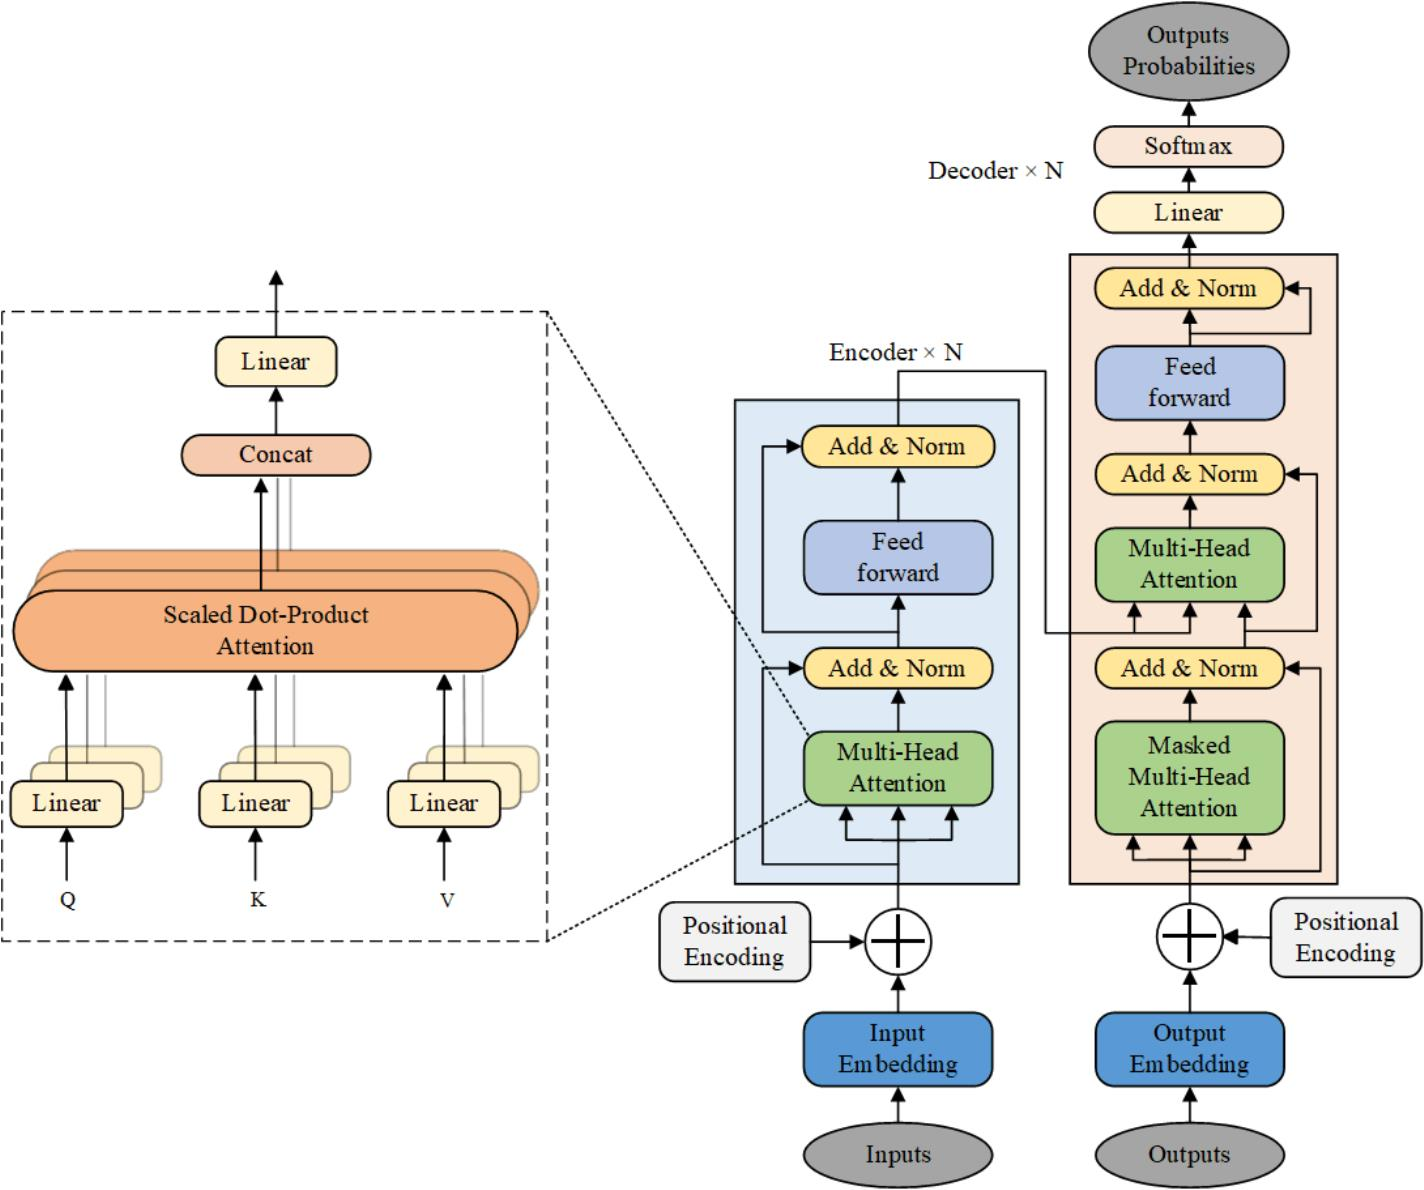
\includegraphics[width=0.75\textwidth]{Transformer}
		\caption{Transformer框架图}
		\label{fig:circuit-diagcam}
	\end{figure}
	Transformer 由编码器(Encoder)和解码器(Decoder)两部分组成,其中编码器将输入序列转换为一系列高维向量,解码器则根据编码器的输出和之前的预测逐步生成目标序列。编码器和解码器都由多层 Transformer    块组成。其中编码器每层由两个子层组成,分别是多头自注意力机制(Multi-Head Self-Attention)和按位置排列的全连接前馈神经网络(Feed-Forward Neural Network)。解码器每层包含3个子层,其中后2个子层结构与编码器子层结构相似,第1个子层对编码器部分的输入进行处理。与编码器类似,每个子层都采用了一个残差连接,并进行层的归一化。以下对Transformer的重要模块进行介绍:
	\par{}
	\textbf{ 位置编码 }
	位置编码是 Transformer 中一个非常重要的步骤,它能够为输入序列中的每个元素赋予一
	种位置信息,从而使得 Transformer 能够处理序列中的元素的位置信息。位置编码可以通过在
	输入向量中加入一些特定的正弦和余弦函数的组合来实现。
	\par
	\textbf{ 多头自注意力机制 }
	自注意力机制是一种能够学习输入序列中不同位置之间的关系的机制。在每个编码器和解码器的Transformer 块中,多头自注意力机制会将输入序列映射为一个键(Key)、一个查询(Query)和一个值(Value)的三元组,通过计算查询和键的点积得到一个注意力分数向量,再将注意力分数向量与值向量相乘得到自注意力向量。多头自注意力机制则是在这个过程中,将注意力机制分为多个头(Head),分别计算注意力分数向量,并将多个自注意力向量拼接起来,然后通过全连接层来进行降维处理。具体计算公式如下:
	\begin{equation}
		\mathbf{Attention(Q,K,V)}  = \mathbf{softmax(\frac{Q{K}^T}{\sqrt{d_k}} )} \cdot \mathbf{V,}
	\end{equation}
	\begin{equation}
		\mathbf{{head}_i} = \mathbf{Attention(Q{W}^Q_i,	K{W}^K_i,V{W}^V_i),}
	\end{equation}
	\begin{equation}
		\mathbf{MultiHead(Q,K,V)} = \mathbf{Concat(head_1,head_2,...head_h){W}^o,}
	\end{equation}
	其中,Q、K、V分别代表输入序列映射到Query、Key、Value的数据向量,$\mathbf{W}^i_Q、\mathbf{W}^i_K、\mathbf{W}^i_V、\mathbf{W}^O$代表不同的权值矩阵,${head}_i$代表第
	i个头注意力模块计算的分数向量。多头注意力机制可以被理解为一种将原始向量集合映射到多个子空间中,并在每个子空
	间中独立地计算注意力权值的机制。具体地,输入的 Query、Key、Value 向量分别被线性变
	换为多个子空间中的向量,然后在每个子空间中分别进行点积注意力权重计算。最后,将每
	个子空间中得到的注意力信息拼接,再次经过一个线性变换得到最终输出向量。
	\par
	\textbf{ 多头自注意力机制 }
	前馈神经网络是 Transformer 中另一个重要的组件。在每个 Transformer 块中,前馈神经
	网络接受来自多头自注意力机制的输出作为输入,并通过两个线性变换和一个非线性激活函
	数来将其映射为一个新的表示向量。具体可表示为:
	\begin{equation}
		\mathbf{FFN(x)} = \mathbf{max(0,x{W}_1+b_1)W_2+b_2}
	\end{equation}
	其中$\mathbf{{W}_1}$、$\mathbf{{W}_2}$分别代表两种不同的线性函数,$\mathbf{{b}_1}$、$\mathbf{{b}_2}$是两个偏置常量。采用的激活函数为 ReLU函数。
	\par
	\textbf{残差连接和归一化 }
	残差连接是指将输入和输出相加,从而将上一层的信息传递到下一层。层归一化则是在
	每个子层输出前对其进行归一化处理,以防止梯度消失和梯度爆炸问题。具体公式如下所示:
	\begin{equation}
		\mathbf{Outlayer} = \mathbf{LaterNorm(x+Sublayer(x)),}
	\end{equation}
	其中,$\mathbf{LaterNorm}$是层归一化函数,$\mathbf{Sublayer(x)}$表示各子层自己实现的函数。
	\subsubsection{ Fastformer }
	Fastformer是由Transformer改进而来的,它是一种基于附加注意力的高效Transformer模型。在Fastformer中,首先使用附加注意机制来建模全局上下文,然后根据与全局上下文表示的交互进一步转换每个令牌表示。通过这种方式,Fastformer可以以线性复杂度实现有效的上下文建模,其结构图如图9所示:
	\begin{figure}[H]
		\centering
		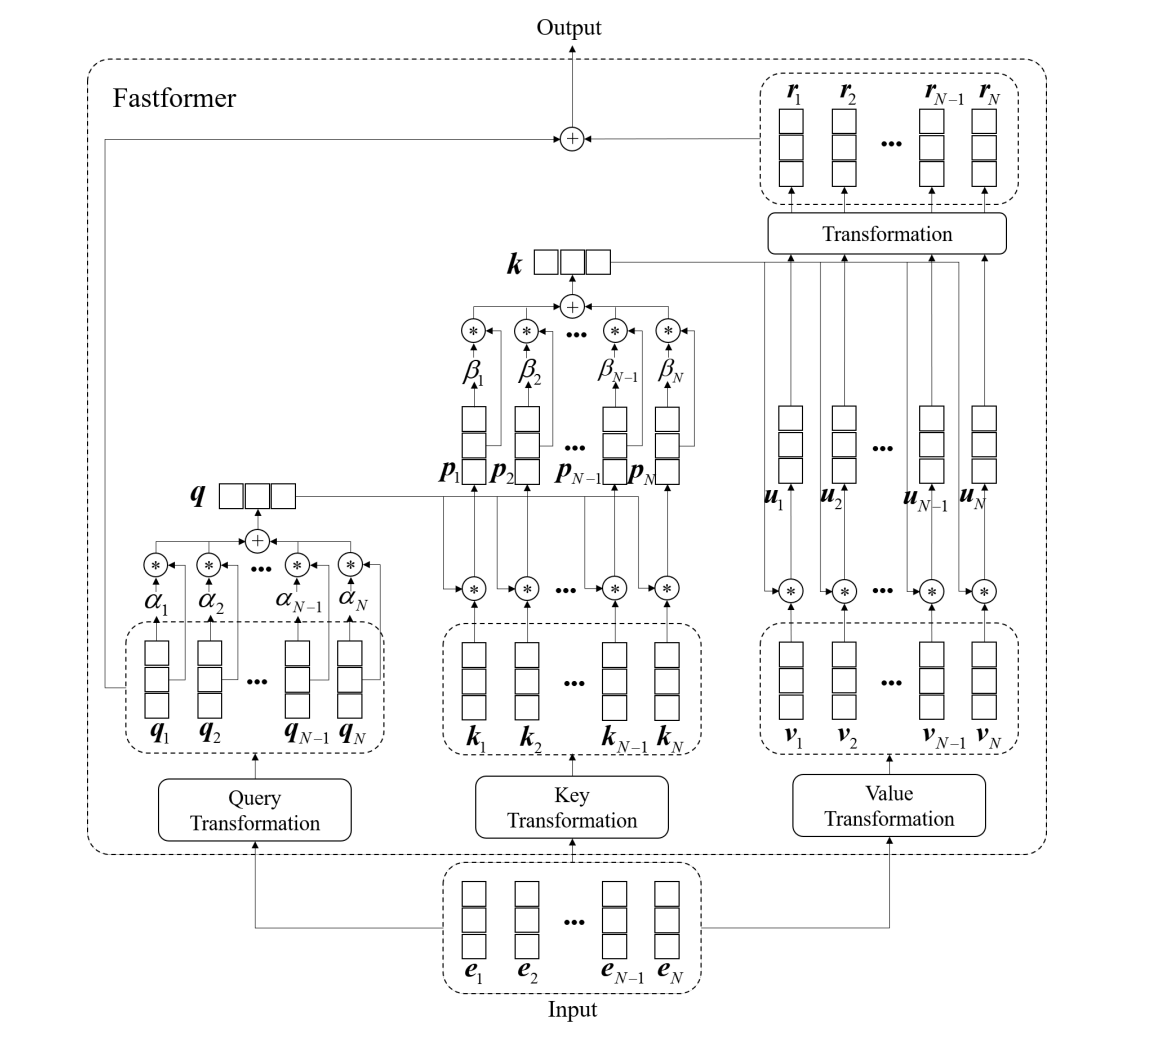
\includegraphics[width=0.8\textwidth]{Fastformer}
		\caption{Fastformer框架图}
		\label{fig:circuit-diagcam}
	\end{figure}
	在Fastformer中,首先使用附加注意机制将输入注意力query矩阵汇总为全局query向量。接下来,通过元素乘积对注意力key和全局query向量之间的交互进行建模,以学习全局上下文感知key矩阵,并通过加性注意力进一步将其汇总为全局key向量。然后使用元素乘积来聚合全局key和注意力值,通过线性变换进一步处理以计算全局上下文感知注意力值。最后,将原始注意力query和全局上下文感知注意力值相加,形成最终输出。这样,计算复杂度可以降低到线性,并且可以有效地捕获输入序列中的上下文信息。在新闻推荐测试推荐的效果,表明Fastformer比许多Transformer模型效率更高,并且可以在长文本建模中取得很好的结果。
	\subsection{模型架构}
	给定用户$u$和候选新闻$n^c$,我们需要计算用户$u$对候选新闻$n^c$内容的兴趣度量相关性分数$z$。然后根据相关性分数对不同候选新闻进行排序并向用户$u$推荐。
	用户$u$与他/她点击的新闻集合$\{ c_1, c_2, \dots, c_m\} $相关,其中$c_i$表示第$i$次点击的新闻,$m$是点击新闻的数量。设$E$表示新闻$c$中的实体。
	我们假设新闻$c$通常会诱导$k$类文本信息(例如标题和实体)$T = \{ T_1, T_2,\dots, T_k\} $,其中$T_i$是新闻文本的第$i$类文本。文本序列$T_i$由多个令牌组成:$T_i = \{ t_{ i,1}  t_{ i,2}  ,\dots, t_{ i,l} \} $,其中$t_{ i,j} $是序列$T_i$中的第{ $j$} 个单词令牌,$l$是序列的最大长度。
	\subsubsection{ 候选新闻编码}
	\textbf{新闻编码器 } 
	为了区分候选新闻和用户点击新闻,我们在候选新闻的相关表示中添加了上标 "c"。
	我们首先将候选新闻文本 $T_i^c$ 中的每个单词 $t^c_{ij}$ 映射到一个 $d_w$ 维的向量 $\mathbf{t}_{ij}^c \in \mathbb{R}^{d_w}$,其中 $d_w$ 是向量维度。因此,文本 $T_i^c$ 可以表示为一个特征图 $\mathbf{T}_i^c = [\mathbf{t}_{i1}^c; \mathbf{t}_{i2}^c; \dots; \mathbf{t}_{il}^c]$,其中 $\mathbf{T}_i^c \in \mathbb{R}^{l \times d_w}$ 。
	Transformer机制基于自注意机制,该机制允许模型权衡序列中不同单词的重要性。它取代了传统的递归神经网络(RNN),在捕捉词与词之间错综复杂的语义和句法关系方面表现出了卓越的性能。因此,我们采用 Transformer 对不同类型的文本信息进行建模。如图所示,第 \textit{i}种类型文本信息的上下文词语的表示 $\hat{\mathbf{T}}_i^c$ 可以表示如下:
	
	\begin{equation}\label{eta}
	\mathbf{\begin{split}
	\hat{\mathbf{t}} _{i1}^{c}, \hat{\mathbf{t}}_{i2}^{c}, \ldots, \hat{\mathbf{t}}_{il}^{c} =\mathrm{Trans} (\mathbf{t}^c_{i1},\mathbf{t}^c_{i2}, \ldots, \mathbf{t}^c_{il})\\
	\hat{\mathbf{T}}_i^c = [\hat{\mathbf{t}}_{i1}^{c}; \hat{\mathbf{t}}_{i2}^{c}; \ldots; \hat{\mathbf{t}}_{il}^{c}]
	\end{split}}
	\end{equation}\label{eta}
	其中 $\hat{\mathbf{T}}^{c}_i \in \mathbb{R}^{l \times d_w}$, 
	第 $i$ 个候选新闻文本 $T_i^c$ 的高级特征向量通过软注意力机制生成: 
	\begin{equation}
	\hat{\mathbf{t}^c_i} = softmax( \mathbf{W} \cdot \mathbf{(\hat{\mathbf{T}}^c_i})^{T} + \mathbf{b}) \cdot \mathbf{\hat{\mathbf{T}}^c_i}
	\end{equation}
	其中,$\hat{\mathbf{t}}^c_i \in \mathbb{R}^{d_w}$, $\mathbf{W}$ 表示可训练的权重矩阵,$\mathbf{b}$ 表示偏差项。
	所有新闻文本的表示被连接起来作为候选新闻的文本表示:
	\begin{equation}\label{eta}
	\mathbf{d}^c= \hat{\mathbf{t}}_1^c \oplus \hat{\mathbf{t}}_2^c \oplus \ldots \oplus \hat{\mathbf{t}}_k^c
	\end{equation}\label{eta}
	其中 $\mathbf{d}^c \in \mathbb{R}^{kd_w}$, $\oplus$ 表示沿行串联向量的操作。\par
	\textbf{知识协同编码器 }
	该编码器旨在借助知识图谱,从用户点击新闻和候选新闻中的实体 $\mathbf{E}^{u} =[E^u_1;E^u_2;\dots;E^u_m] $ 和 $\mathbf{E}^{c} = [E^c_1;E^c_2;\dots;E^c_n] $ 之间的相关性出发,更好地表示这些新闻,以便进行兴趣匹配。该机制包含三个部分。首先,为了总结每个实体或其邻居在跳数范围内的信息,它首先利用图注意(GAT)网络堆叠层来学习它们的表示,分别表示为 $\mathbf{M}_u \in \mathbb{R}^{d_e \times D}$和 $\mathbf{M}_c \in \mathbb{R}^{d_e \times D}$,其中 D 是点击新闻和候选新闻中实体的数量。
	
	其次是堆叠图共注意力(GCAT)网络。一般来说,一个实体通常与知识图谱上的多个实体具有丰富的关联性。而且,实体间的相关性通常会提供不同的信息用以建模点击新闻和候选新闻之间的相关性,从而进行兴趣匹配。为了更好地选择实体间信息的相关性来匹配用户感兴趣的候选新闻,我们提出了一种堆叠了 K 层的图协同关注网络(GCAT)来学习新闻 $ {n}^{u}$ 和 ${n} ^ {c} $ 中实体的匹配感知表示。以新闻 $ {n}^{u} $ 和 $l$-th 图共注意力网络中的实体 e 为例,我们首先将多头自注意力网络应用于由第 $l-1$ 个 GCAT 网络生成的其相邻实体的表征,以建模不同相邻实体之间的相关性。接下来,我们提出了一个匹配感知注意力网络,根据实体e与新闻${n}^{c}$中实体的相关性来聚合实体e的邻居实体,相关性矩阵$ \mathbf{I}_u \in \mathbb{R}^{D \times B} $:
	\begin{equation}
	\mathbf{I}_u = \mathbf{M^T_c} \mathbf{W^c_c} \hat{\mathbf{G}_l}
	\end{equation}
	其中 $\hat{\mathbf{G}_l} \in \mathbb{R}^{d_e \times
	B}$表示自注意力网络生成的邻居实体的表示,B 表示邻居的数量,$\mathbf{W}^c_c$是可训练的权重。邻居实体的注意力向量 $\mathbf{v}^{u} \in \mathbb{R}_B $ 的计算公式为:
	\begin{equation}
	\mathbf{v}^{u} = \mathbf{q}^T_e \cdot tanh(\mathbf{W}^c_s \hat{\mathbf{G}^{l}} + \mathbf{W}^c_h \mathbf{M}_c f(\mathbf{I}_u) ), 
	\end{equation}
	其中,f 代表softmax激活函数,它对输入矩阵的每列向量进行归一化处理,$\mathbf{q}_e$ 表示可训练的注意力查询矩阵,$\mathbf{W}^c_s$ 和 $\mathbf{W}^c_h$ 是可训练的权重矩阵。
	然后,我们将实体 e 的邻居聚合到一个统一的表示 $\hat{\mathbf{g}^{l}} \in \mathbb{R}^{\mathbf{d}_e}  $:
	\begin{equation}
	\hat{\mathbf{g}^{l}} = \sum_{i=1}^{B}\mathbf{\lambda}^u_i\hat{\mathbf{g}^l_i},{~~~~~~~~}      
	\mathbf{\lambda}^u_i = \frac{exp(\mathbf{v}^u_i)}{\sum_{j=1}^{B}exp(\mathbf{v}^u_j)}
	\end{equation}
	其中,$\mathbf{v}^u_i$ 是向量$v^u$ 的第 i 个元素,$\mathbf{\lambda}^u_i$为第 i 个邻居实体的注意力权重。第 $l$ 个 GCAT 网络生成的实体 e 的表示$g^l$为:$g^l = \mathbf{P}_e[\hat{\mathbf{g}^{l}};\hat{\mathbf{g}}^{l-1}]$,其中,$P_e\in \mathbb{R}^{d_e\times2d_e}$为投影矩阵。采用这种方法,堆叠了 K 层的 GCAT 网络就可以通过捕捉 K 跳内的邻居与候选新闻中的实体之间的相关性,为用户点击新闻中的实体学习匹配感知表示 $S_u \in \mathbb{R}^{d_e \times D}$。 以类似的方式,我们可以通过候选新闻中实体的邻居与点击新闻中实体之间的相关性来学习候选新闻中实体的匹配感知表示 $S_c \in \mathbb{R}^{d_e \times D}$。
	
	第三个是实体共同注意力网络。点击新闻和候选新闻中的实体通常具有不同的信息用于兴趣匹配。
	我们应用实体共同注意力网络,通过捕捉实体之间的相关性,交互式地学习新闻 $n^u$ 和 $n^c$ 的知识型表示。具体来说
	首先,我们计算一个亲和矩阵来衡量新闻 $n^u$ 和 $n^c$ 中实体之间的相关性:
	\begin{equation}
	\mathbf{C}_e = \mathbf{S}^T_c\mathbf{W}^K_c\mathbf{S}_u,
	\end{equation}
	其中 $\mathbf{W}^c_k \in \mathbb{R}^{d_e \times d_e}$是权重矩阵。接下来我们计算新闻 $n^u$ 和 $n^c$ 中实体的注意力向量 $a^u,a^c \in \mathbb{R}^{D}$,并且将矩阵 $C_e$ 和 $C^e_T$ 作为相关矩阵,计算点击新闻和候选新闻中基于知识的表示 $u_e \in \mathbb{R}^{d_e}$ 和 $c_e \in \mathbb{R}^{d_e}$ ,它可以通过公式(5)和(6)进行计算。我们将候选新闻的文本表征和实体表征融合为候选新闻表征:
	\begin{equation}
	\mathbf{n^c}=\mathbf{d}^c \oplus \mathbf{c_e}
	\end{equation}
	其中,$\mathbf{n^c \in \mathbb{R}^{kd_w+D}}$, 获取的候选新闻表示将后续阶段将用于进行用户兴趣建模和匹配。
	\subsubsection{ 单词粒度感知候选新闻}
	本部分旨在将候选新闻特征纳入用户点击历史新闻词级表示中。
	具体来说,将 第$i$ 个新闻文本 $T_i$ 中的每个单词 $t_{ij}$ 映射为一个 $d_w$ 维向量 $\mathbf{t}_{ij} \in \mathbb{R}^{d_w}$,我们就可以得到表示矩阵  $T_i$ : $\mathbf{T}_i = [\mathbf{t}_{i1}; \mathbf{t}_{i2}; \dots; \mathbf{t}_{il}]$,其中 $\mathbf{T}_i \in \mathbb{R}^{l \times d_w}$ 。
	不同类型的新闻文本通常具有不同的语义特征,这对新闻语义理解非常重要。 因此,用户点击新闻的表示矩阵被堆叠成一个总矩阵 $\mathbf{T}$:$\mathbf{T} =[\mathbf{T} _1^1;\ldots;\mathbf{T} _k^1;\ldots;\mathbf{T} _1^m;\ldots;\mathbf{T} _k^m]$、其中 $\mathbf{T} \in \mathbb{R}^{mkl \times d_w}$, $\mathbf{T}_j^i$ 是第 $i$  个点击新闻 $c_i$ 的第 $j$ 个新闻文本嵌入矩阵。为方便起见,我们将 $\mathbf{T}$ 重写如下:
	\begin{equation}
	\mathbf{G} = [\mathbf{g}_1; \mathbf{g}_2, \dots, \mathbf{g}_L],~~ \mathbf{G} \in \mathbb{R}^{L\times d_w},~~L = mkl
	\end{equation}
	其中,$\mathbf{g}_i$ 是点击新闻整体序列的第 $i$ 个单词表示向量。
	尽管Transformer网络被公认为是一种强大的文档建模方法,但由于其二次方的复杂度,它在处理长文档时的效率大打折扣。受此启发,我们采用了 Fastformer(一种 SOTA 高效transformer网络)来对用户点击的长新闻进行单词级行为交互建模。 Fastformer 的核心组件是加性注意力机制,它能够在线性复杂度下实现有效的上下文建模。为了有效地学习候选新闻与点击新闻在单词层面的交互,我们设置每个词头的查询($\mathbf{q}_i$)、关键字($\mathbf{k}_i$)和值($\mathbf{v}_i$)计算如下:	
	\begin{equation}
	\mathbf{q}_i = W^w_q(\mathbf{g}_i \oplus \mathbf{n^c}),~~
	\mathbf{k}_i = W^w_k\mathbf{g}_i,~~
	\mathbf{v}_i = W^w_v\mathbf{g}_i
	\end{equation}
	其中,$W^w_q$、$W^w_k$、$W^w_v$ 表示可训练的投影参数矩阵。候选新闻感知表示 $\hat{\mathbf{g}}_i$ 的计算方法如下:
	% Each query incorporate the candidate news information, which can guide the model learn the important information. 
	\begin{equation}\label{wcan}
	\begin{split}
	\mathbf{q} = Att(\mathbf{q}_1, \mathbf{q}_2, \dots, \mathbf{q}_L)\\
	\mathbf{k} = Att(\mathbf{q} * \mathbf{k}_1, \mathbf{q} * \mathbf{k}_2, \dots, \mathbf{q} * \mathbf{k}_L)\\
	\hat{\mathbf{g}}_i = \mathbf{W}_o(\mathbf{k} * \mathbf{v}_i)
	\end{split}
	\end{equation}
	其中,``$*$" 表示两个矩阵对应位置元素进行乘积, $Att(\cdot)$ 表示池化注意力网络,$\mathbf{W}_o$ 表示可训练参数矩阵。随后,不同注意力头的输出被连接起来,为第i个文本构建一个统一的上下文表示,即 $\bar{\mathbf{g}}_i$ 。我们让  $\bar{\mathbf{G}}= [\bar{\mathbf{g}}_1,\bar{\mathbf{g}}_2, \ldots,  \bar{\mathbf{g}} _L]$ 。
	 因此,单词级的用户兴趣表示 $\mathbf{u}_w$ 可以计算如下:
	\begin{equation}
	\mathbf{u} _w = softmax( \mathbf{W} \cdot \mathbf{\bar{G}}^{T} + \mathbf{b}) \cdot \mathbf{\bar{G}}
	\end{equation}
	\subsubsection{ 实体粒度感知候选新闻 }
	该机制旨在通过将候选新闻纳入实体表征来为用户兴趣建模。我们首先得到所有点击新闻和候选新闻的知识增强实体表示 $\mathbf{E}^{u} = [E^u_1;E^u_2;\dots;E^u_m] $ 和 $\mathbf{E}^{c} = [E^c_1;E^c_2;\dots;E^c_n] $。m 和 n 是点击新闻和候选新闻的数量。然后,我们使用知识感知新闻协同编码器(Knowledge-aware News Co-Encoder)获得实体级用户兴趣表示 $\mathbf{u}_e $.
	\subsubsection{ 新闻粒度感知候选新闻}
	在这一部分 
	我们首先通过新闻编码器获取点击新闻的表示$\mathbf{d}=[\mathbf{d}_1, \mathbf{d}_2,\dots,\mathbf{d}_m]$,其中$\mathbf{d}_i \in \mathbb{R}^{kd_w}$表示第$i$个用户点击新闻的向量表示。
	然后,利用Transformer从用户点击的新闻中捕捉交互信息。
	多头自注意力机制单元是 Transformer 的主要组成部分。
	与传统 Transformer 不同,对于多头自关注机制中的每个头,我们设置查询、键和值如下:
	\begin{equation}\label{eatt}
	\mathbf{q}_{i} = \mathrm{ReLU}((\mathbf{d}_i \oplus \mathbf{n}^c) \cdot W^n_q),~ \mathbf{k}_{i} = \mathrm{ReLU}(\mathbf{d}_i \cdot W^n_k),~
	\mathbf{v}_{i} = \mathrm{ReLU}(\mathbf{d}_i \cdot W^n_v)
	\end{equation}
	其中,$W^n_q$、$W^n_k$ 和 $W^n_v$ 分别是查询、键和值的可学习权重矩阵。对于每条新闻 $c_i$,自注意力机制会学习一组权重 $\beta_i = \{\beta_{i1}, \beta_{i2}, \dots, \beta_{im}\}$,用于衡量所有被点击的新闻 \{$c_1$,$c_2$,$\dots$,$c_m$\}回答查询 $\mathbf{q}_i$ 的程度:
	\begin{equation}
	\beta_{ij} = \frac{q_ik_j}{\sum_{j'}exp(q_ik_{j'})}
	\end{equation}
	输出结果是所有新闻的加权和:
	\begin{equation}
	f_i = \sum_j \beta_{i,j}v_j
	\end{equation}
	之后,我们将不同注意力头的输出串联起来,形成统一的上下文表示,并进一步输入前馈网络。然后每个新闻表征可以得到 $\mathbf{f}_i \in \mathbb{R}^{d_n}$,其中 $d_n$ 是向量维度。新闻级用户兴趣表征的总矩阵为 $\mathbf{F}=[\mathbf{f}_1; \mathbf{f}_2; \cdots; \mathbf{f}_m]$,其中 $\mathbf{F} \in \mathbb{R}^{m \times d_n}$.
	最后,新闻层面的用户兴趣表示可以计算如下:
	\begin{equation}
	\mathbf{u}_n = softmax( \mathbf{W} \cdot \mathbf{F}^{T} + \mathbf{b}) \cdot \mathbf{F}
	\end{equation}
	其中,$\mathbf{u}_n$ 表示新闻层面的用户兴趣表示,$\mathbf{W}$ 表示可训练的权重矩阵,$\mathbf{b}$ 表示偏差项。
	候选新闻和用户点击新闻之间不同粒度的交互对于用户兴趣建模非常重要。因此,我们将单词级、实体级和新闻级的候选感知用户兴趣表示聚合起来,作为最终的用户兴趣特征:
	\begin{equation}
	\mathbf{u} = [\mathbf{u}_w; \mathbf{u}_e; \mathbf{u}_n]
	\end{equation}
	沿袭前人的研究成果,我们采用候选新闻感知用户表示 $\mathbf{u}$ 和候选新闻表示 $\mathbf{n}^c$ 的点积来衡量用户兴趣和候选新闻的相关性: $\hat{y} = \mathbf{u}^T \cdot \mathbf{n}^c$。然后根据匹配分数 $\hat{y}$ 对候选新闻进行排序,以推荐新闻。接下来我们将介绍为实现所提方法而使用的训练方法。我们利用负抽样技术来构建训练数据集 $\mathcal{D}$,其中每个正样本都与从同一新闻中随机抽取的 $\mathcal{S}$ 负样本相关联。
	此外,我们还应用了 BPR 损失来制定损失函数:
	\begin{equation}\label{eatt}
	\mathcal{L} =- \frac{1}{|D|}  {\textstyle \sum_{i=1}^{|D|}{\sigma (y_i^c-y_i^n)}}
	\end{equation}
	其中,$\sigma$ 是激活函数、
	$y_i^c$ 和 $y_i^n$ 是第 $i$ 个已点击和未点击新闻样本的匹配得分。
	\newpage
	\subsection{模型评估}
	\subsubsection{与之前的模型指标对比}
	\begin{table}[h]
		\centering
		\caption{MGCA与之前模型的对比}
		\setlength{\tabcolsep}{7mm}{
			\begin{tabular}{lcccc}
				\hline
				模型 & AUC & MRR & nDGG@5 & nDGG@10 \\
				\hline
				DAN & 65.14 & 30.04 & 32.98 & 39.52 \\
				NAML & 64.21 & 29.71 & 32.51 & 39.00 \\
				NPA & 63.71 & 29.84 & 32.40 & 39.02 \\
				LSTUR & 65.51 & 30.22 & 33.26 & 39.76 \\
				NRMS & 65.36 & 30.02 & 33.11 & 39.61 \\
				FIM & 64.46 & 29.52 & 32.26 & 39.08 \\
				KRED & 65.61 & 30.63 & 33.80 & 40.23 \\
				KIM & 67.13 & 32.08 & 35.49 & 41.79 \\
				FUM & 66.81 & 31.37 & 34.81 & 41.22 \\
				\hline
				MGCA & \textbf{68.13} & \textbf{33.41} & \textbf{36.12} & \textbf{42.75} \\
				\hline
		\end{tabular}}
	\end{table}
	\subsubsection{消融实验}
	\begin{table}[h]
		\centering
		\caption{ 消融实验结果}
		\label{resultecsp}
		\setlength{\tabcolsep}{5.5mm}{
			\begin{tabular}{lcccc}
				\hline
				模型 & AUC & MRR & nDGG@5 & nDGG@10 \\
				\hline
				\textbf{去除单词级粒度} & 63.76 &	31.12 &	33.80 &	40.68\\
				\textbf{去除单词级感知} &67.34 &	31.71 &	34.43 &	40.67 \\
				\textbf{去除新闻级粒度} &64.34 &	30.95 &	33.66 &	40.87\\
				\textbf{去除新闻级感知} & 65.26 &	30.19 &	33.44 &	39.92\\
				\textbf{去除实体级粒度} & 67.24 &	31.37 &	34.15 &	40.54  \\
				\textbf{去除实体级感知} & 65.14 &	31.22 &	33.53 &	39.60  \\
				\textbf{去除所有感知} & 64.39 &	30.09 &	33.18 &	40.16 \\
				\hline
				\textbf{MGCA} & \textbf{68.13} & \textbf{33.41} & \textbf{36.12} & \textbf{42.75} \\
				\hline
		\end{tabular}}
	\end{table}
	\newpage
	\section{软件工程与开发架构方案}
	\subsection{开发工具与框架}
	系统开发操作系统环境:Windows11\par
	数据库:MySql\par
	开发语言:JAVA,Python\par
	JDK:jdk1.8\par
	Python:3.6\par
	开发平台:InteliJ IDEA 2022.1.3\par
	前端框架:Vue3,bootstrap\par
	后端框架:springboot
	\subsection{新闻推荐系统软件落地示例}
	\subsubsection{ 软件周期模型}
	在软件周期模型阶段,我们将采用经典的软件开发周期,包括可行性分析、需求分析、设计、开发、测试和部署等阶段。在可行性分析阶段,我们将对新闻网站个性化推荐系统的可行性进行评估,以确定项目是否值得投入,并识别潜在的风险和挑战。在需求分析阶段,我们将利用敏捷开发方法论,通过迭代方式逐步完善前端与后端的功能。在设计阶段,我们将着重考虑系统架构和界面设计,确保软件具备良好的可扩展性和用户体验。在开发阶段,我们将按照设计方案进行编码和实现,并且进行代码审查以确保代码质量。在测试阶段,我们将进行单元测试、集成测试和系统测试,以发现和修复可能存在的问题。最后,在部署阶段,我们将准备好软件的发布版本,并进行部署和配置,确保软件能够正常运行并满足用户需求。
	\textbf{(1)可行性分析阶段}\par
	项目面临着一些技术挑战,包括评估网站新闻个性化推荐算法的复杂性和实现难度,以及与多个数据源对接的挑战。为了应对这些难题,我们将记录用户历史点击新闻,并将其与候选新闻输入到算法中,通过智能计算得到匹配度,以优先显示匹配度较高的新闻。市场调研表明,在当前信息过载的环境下,一套个性化新闻推荐系统更符合市场需求且具有竞争优势。在成本估算方面,我们将综合考虑项目开发、运维、推广等各方面的成本,包括硬件、软件、人力等,以确定项目值得投入的程度。
	\par
	\textbf{(2)需求分析阶段}\par
	随着互联网的高速发展,信息量呈爆炸式增长,用户逐渐由信息匮乏时代迈入信息过载时代。在这样的背景下,我们的目标是建立一个新闻网站,通过个性化推荐系统帮助用户从海量信息中快速准确地找到感兴趣的内容,提高用户体验、用户数量和用户粘性。\par
	$\bigstar$个性化推荐: 根据用户的历史浏览记录、点击行为、点赞收藏等个性化信息,推荐用户感兴趣的新闻内容。\par
	$\bigstar$实时更新:系统需要能够实时从各个新闻源获取最新的新闻内容,并将其纳入推荐范围。\par
	$\bigstar$多样化推荐算法:结合协同过滤、内容分析、深度学习等技术,提供多种推荐算法,确保推荐结果的准确性和多样性。\par
	$\bigstar$用户反馈机制:提供用户反馈功能,用户可以对推荐结果进行点赞、收藏、举报等操作,以优化推荐算法。\par
	$\bigstar$个人信息管理:提供用户个人信息管理功能,用户可以编辑个人兴趣标签、设置推送频率等。\par
	$\bigstar$跨平台兼容性:支持多平台访问,包括PC端、移动端和平板电脑端,保证用户在不同设备上的使用体验一致。\par
	\textbf{(3)设计阶段}\par
	新闻推荐系统分为用户管理模块、新闻管理模块、数据处理模块和推荐算法模块。如图所示,用户管理模块主要负责对用户信息的管理,用户管理模块是新闻推荐系统中的重要功能模块之一,主要负责对用户信息的管理,包括用户的注册、登录、用户信息管理等功能。新闻管理模块包括新闻的采集、存储以及新闻的更新管理等功能。数据处理模块在处理新闻内容以及用户行为产生的数据后,将会对数据进行数据清洗和分析,处理后的结果将会存储在数据库中。推荐算法构建推荐系统模块在已有数据的基础上构建推荐算法,基于数据进行分析,根据推荐算法得出对目标用户的推荐结果,并向用户推送。\par
	\begin{figure}[H]
		\centering
		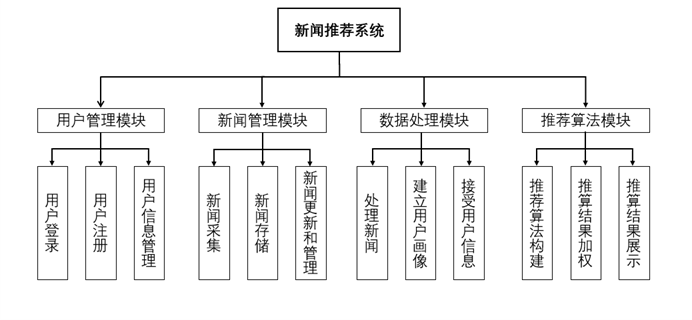
\includegraphics[width=0.95\textwidth]{系统功能模块图}
		\caption{系统功能模块}
		\label{fig:circuit-diagcam}
	\end{figure}
	\textbf{(4)测试阶段}\par
	在测试阶段,我们将进行系统的测试以确保其质量和稳定性,通过单元测试、集成测试和系统测试对系统进行正向测试。通过漏洞扫描对系统进行逆向测试,保障系统的安全性,通过授权和认证测试,测试系统的用户授权和认证机制。\par
	$\bigstar$单元测试: 对系统中的各个单元(函数、模块)进行测试,验证其功能的正确性。\par
	$\bigstar$集成测试:将系统中各个单元集成在一起,测试其之间的交互和整体功能。\par
	$\bigstar$系统测试:对整个系统进行端到端的测试,模拟用户使用场景,验证系统的功能和性能。\par
	$\bigstar$漏洞扫描:使用安全扫描工具对系统进行扫描,发现并修复潜在的安全漏洞。\par
	$\bigstar$授权和认证测试:测试系统的用户授权和认证机制,确保用户的身份和权限受到正确的控制。
	\subsubsection{ 软件开发模型}
	在软件开发过程中,我们选择了原型开发模型作为主要的软件开发模型。原型开发模型将软件功能划分为多个增量,每个增量都包含一个或多个功能模块,可以独立开发、测试和部署。通过采用原型开发模型,我们能够快速地推出部分功能,并根据用户反馈和需求变化进行灵活调整和优化,从而逐步完善和扩展整个系统。同时,我们也将结合敏捷开发方法论,注重团队协作、持续交付和快速响应变化,以确保项目能够及时交付高质量的软件产品。下面是新闻推送系统的主要功能,通过良好的用户管理,新闻个性化推送等功能提高系统的安全性、用户体验和用户参与度,为用户提供更好的服务。\par
	\textbf{(1)用户注册与登录功能}\par
	在用户注册时,允许用户填写必要的信息进行注册,包括用户名、密码、邮箱等。对用户输入的注册信息进行合法性验证,确保信息的准确性和完整性。在用户注册成功后,将生成唯一的用户ID及用户的个人信息加密处理,并保存到数据库中。提供用户登录界面,用户输入用户名和密码进行登录,对用户输入的登录信息进行验证,确保用户身份的合法性。\par
	\textbf{(2)用户信息管理与权限管理功能}\par
	允许用户在登录后查看和编辑个人信息,包括用户名、密码、邮箱、个人简介等,提供修改密码、修改邮箱等功能,确保用户信息的安全和隐私。区分不同用户的权限等级,如普通用户、管理员等。管理员具有对用户信息的更高权限,可以对用户进行管理和审核。\par
	\textbf{(3)新闻呈现功能}\par
	新闻呈现模块负责将系统中的新闻内容以合适的方式呈现给用户,以便用户浏览和阅读。进行新闻分类与标签,将新闻按照不同的分类和标签进行归类,方便用户根据兴趣进行浏览和筛选。在首页或特定页面展示新闻列表,包括最新新闻、热门新闻、推荐新闻等,以吸引用户点击和阅读。提供详细的新闻内容展示页面,包括新闻标题、内容、作者、发布时间等信息,以及相关的图片、视频等多媒体内容。允许用户通过关键词搜索查找感兴趣的新闻内容,提高用户检索效率。记录用户浏览过的新闻内容,方便用户查看和回顾之前的阅读历史。\par
	\begin{figure}[H]
		\centering
		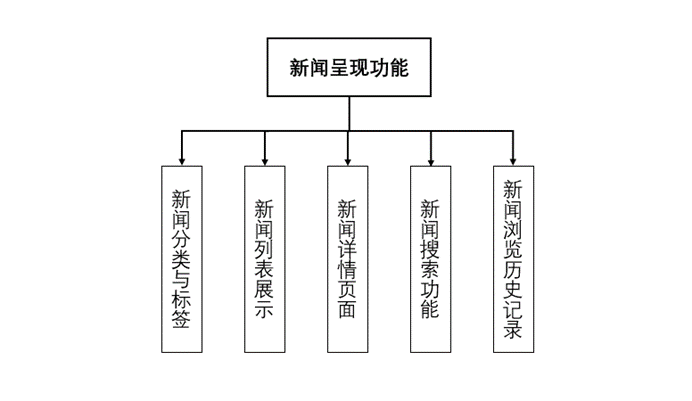
\includegraphics[width=0.75\textwidth]{新闻呈现功能详细框图}
		\caption{新闻呈现功能详细框图}
		\label{fig:circuit-diagcam}
	\end{figure}
	\textbf{(4)用户行为记录功能}\par
	用户行为记录模块用于跟踪和记录用户在系统中的行为,包括浏览、点赞、收藏、评论等操作,以便系统能够更好地理解用户的兴趣和偏好,为个性化推荐提供数据支持。记录用户浏览过的新闻内容,包括浏览时间、浏览时长等信息。记录用户对新闻内容进行点赞和收藏的行为,以及取消点赞和取消收藏的操作。记录用户对新闻内容进行评论的内容和时间,以及评论的回复和删除等操作。\par
	\begin{figure}[H]
		\centering
		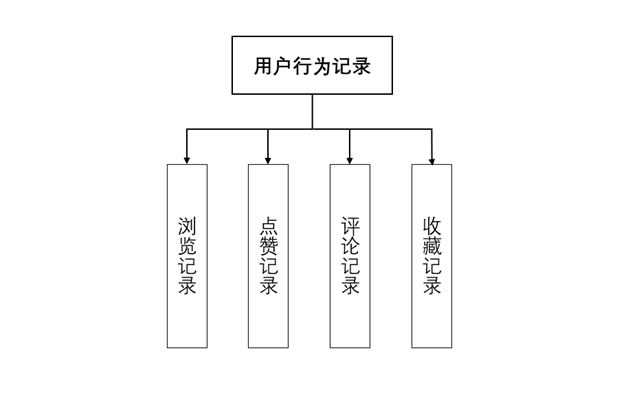
\includegraphics[width=0.75\textwidth]{用户行为记录详细框图}
		\caption{用户行为记录详细框图}
		\label{fig:circuit-diagcam}
	\end{figure}
	\textbf{(5)新闻个性化推送功能}\par
	新闻个性化推送功能根据用户的历史行为和偏好,向用户推荐感兴趣的新闻内容,提高用户的阅读体验和满意度。结合用户的浏览历史、点赞收藏记录等数据,采用推荐算法为用户推荐符合其兴趣的新闻内容。将个性化推荐的新闻内容展示在用户的首页或推荐页面,以便用户方便浏览和阅读。实时更新推荐结果,根据用户的实时行为和偏好,动态调整和更新推荐结果,确保推荐内容的时效性和准确性。\par
	\begin{figure}[H]
		\centering
		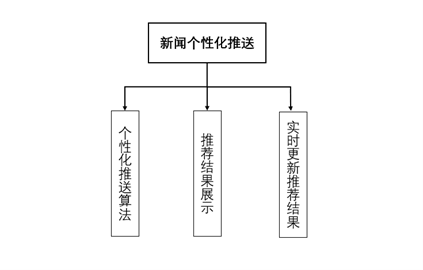
\includegraphics[width=0.75\textwidth]{个性化推荐功能详细框图}
		\caption{个性化推荐功能详细框图}
		\label{fig:circuit-diagcam}
	\end{figure}
	\subsubsection{ 数据库设计}
	\textbf{1.数据库概念结构设计}\par
	概念设计是独立于数据库管理系统的设计,主要完成对现实事物、事物关系之间的转化,把抽象的事物转化成能够被人们易于理解的图形关系,更加直白的把现实的事物关系表达出来,从而为下一步的设计打下一个良好的基础。识别新闻推荐系统中的实体,识别实体的属性,识别实体的关键字,识别实体间的联系,利用实体关系图(E-R图)来描述新闻推荐系统相关实体、属性及关系,从而达到为水果零售超市管理系统建立良好的数据模型的目的。\par
	新闻推荐系统中有用户实体,历史点击新闻实体和候选新闻实体,用户通过点击收藏等行为产生历史点击新闻记录,系统的候选新闻通过与历史点击新闻进行算法计算,得出与近期用户点击新闻的匹配度,然后再将匹配度高的新闻推荐给用户。\par
	\begin{figure}[H]
		\centering
		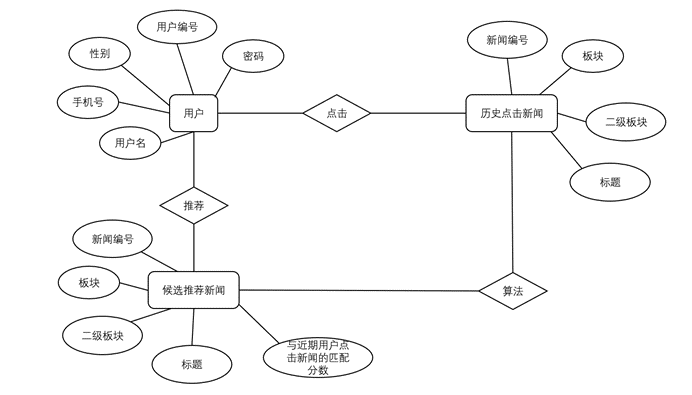
\includegraphics[width=1.00\textwidth]{总体E-R图设计}
		\caption{总体E-R图设计}
		\label{fig:circuit-diagcam}
	\end{figure}	
	\textbf{2.数据库逻辑结构设计}\par
	根据关系数据库逻辑设计的步骤首先将概念模型E-R图转换为关系模式的集合,得到关系数据库模式;然后运用关系数据理论对关系数据库模式进行规范化处理。由概念模型转化为逻辑模型,每个用户对应多个历史点击新闻和多个候选推荐新闻,为每个用户建立一个历史点击新闻数据表和一个候选新闻推荐表。用户关系有用户编号、用户名、手机号、密码和性别等属性,其中用户编号是关系的主键。候选推荐新闻关系有新闻编号、板块、二级板块、标题和与近期用户点击新闻的匹配分数等属性,其中新闻编号是关系的主键。历史点击新闻关系有新闻编号、板块、二级板块和标题等属性,其中新闻编号是关系的主键。\par
	用户(用户编号,用户名,手机号,密码,性别)\par
	候选推荐新闻(新闻编号,板块,二级板块,标题,匹配分数)\par
	历史点击新闻(新闻编号,板块,二级板块,标题)\par
	\begin{figure}[H]
		\centering
		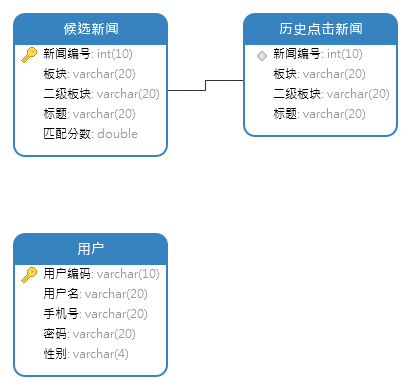
\includegraphics[width=0.55\textwidth]{逻辑结构设计}
		\caption{逻辑结构设计}
		\label{fig:circuit-diagcam}
	\end{figure}		
	\textbf{3.数据库物理结构设计}\par
	\begin{table}[!ht]
		\centering
		\caption{用户关系主码及属性设计}
		\begin{tabular}{|l|l|l|l|l|l|}
			\hline
			\textbf{名} & \textbf{类型} & \textbf{长度} & \textbf{Not Null} & \textbf{键} & \textbf{注释 } \\ \hline
			用户编号 & int & 10 & TRUE & TRUE & 用户的唯一编号  \\ \hline
			用户名 & varchar & 20 & TRUE & FALSE & 用户的名字  \\ \hline
			手机号 & varchar & 20 & TRUE & FALSE & 用户的手机号  \\ \hline
			密码 & varchar & 20 & TRUE & FALSE & 用户设置的登录口令  \\ \hline
			性别 & varchar & 4 & TRUE & FALSE & 只能填写男或女  \\ \hline
		\end{tabular}
	\end{table}
	
	\begin{table}[!ht]
		\centering
		\caption{候选推荐新闻主码及属性设计}
		\begin{tabular}{|l|l|l|l|l|l|}
			\hline
			\textbf{名} & \textbf{类型} & \textbf{长度} & \textbf{Not Null} & \textbf{键} & \textbf{注释 } \\ \hline
			新闻编号 & int & 10 & TRUE & TRUE & 新闻的唯一编号  \\ \hline
			板块 & varchar & 20 & TRUE & FALSE & 新闻对应的一级板块  \\ \hline
			二级板块 & varchar & 20 & FALSE & FALSE & 新闻对应的二级板块  \\ \hline
			标题 & varchar & 20 & TRUE & FALSE & 新闻的标题  \\ \hline
			匹配分数 & double & ~ & TRUE & FALSE & 与近期用户点击新闻的匹配分数  \\ \hline
		\end{tabular}
	\end{table}
	
	\begin{table}[!ht]
		\centering
		\caption{候选推荐新闻主码及属性设计}
		\begin{tabular}{|l|l|l|l|l|l|}
			\hline
			\textbf{名} & \textbf{类型} & \textbf{长度} & \textbf{Not Null} & \textbf{键} & \textbf{注释 } \\ \hline
			新闻编号 & int & 10 & TRUE & TRUE & 新闻的唯一编号  \\ \hline
			板块 & varchar & 20 & TRUE & FALSE & 新闻对应的一级板块  \\ \hline
			二级板块 & varchar & 20 & FALSE & FALSE & 新闻对应的二级板块  \\ \hline
			标题 & varchar & 20 & TRUE & FALSE & 新闻的标题  \\ \hline
		\end{tabular}
	\end{table}
	
	
	
	
	\subsubsection{ UML设计}
	在本项目中,我们采用 UML 来进行系统的设计和建模。通过使用 UML,我们可以清晰地表达系统的功能、组件、交互关系和行为,为系统开发提供了一个统一的设计语言和工具。在UML设计中,我们主要采用用例图、类图、时序图、架构图等图表。\par
	用例图用于描述系统的功能和用户之间的交互关系,显示了系统的外部行为和功能。通过用例图,我们可以清晰地识别新闻推荐系统的主要功能和用户需求,可知普通用户通过登录后可进入系统查看新闻消息,通过并确定系统的边界和范围。\par
	\begin{figure}[H]
		\centering
		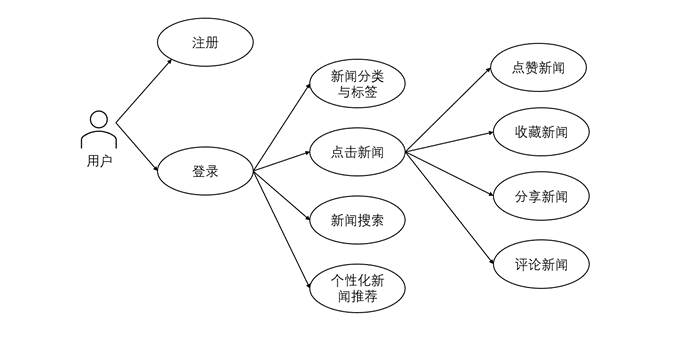
\includegraphics[width=0.95\textwidth]{用例图(普通用户)}
		\caption{用例图(普通用户)}
		\label{fig:circuit-diagcam}
	\end{figure}
	\begin{figure}[H]
		\centering
		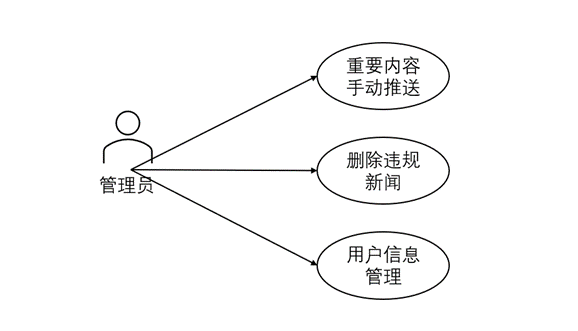
\includegraphics[width=0.65\textwidth]{用例图(管理员)}
		\caption{用例图(管理员)}
		\label{fig:circuit-diagcam}
	\end{figure}
	
	类图用于描述系统的静态结构,包括类、属性、方法和它们之间的关系。类图展示了系统中各个类之间的继承、关联、聚合等关系,帮助开发团队理解系统的组织结构和数据模型。时序图用于描述系统的动态行为,展示了对象之间的消息传递和交互顺序。时序图可以清晰地展现系统中各个对象之间的交互过程和消息传递顺序,帮助开发团队理解系统的执行流程和时序关系。\par
	通过使用这些 UML 图表,我们可以全面、清晰地描述系统的结构和行为,为开发团队提供了一个统一的设计和沟通语言,帮助团队成员更好地理解和协作,从而有效地完成项目开发任务。\par
	
	\subsubsection{ 软件功能演示}
	在软件功能演示阶段,我们将对新闻推荐系统的各项功能进行演示展示,包括用户注册登录、新闻内容浏览、个性化推荐等功能。\par
	1.用户注册页面\par
	\begin{figure}[H]
		\centering
		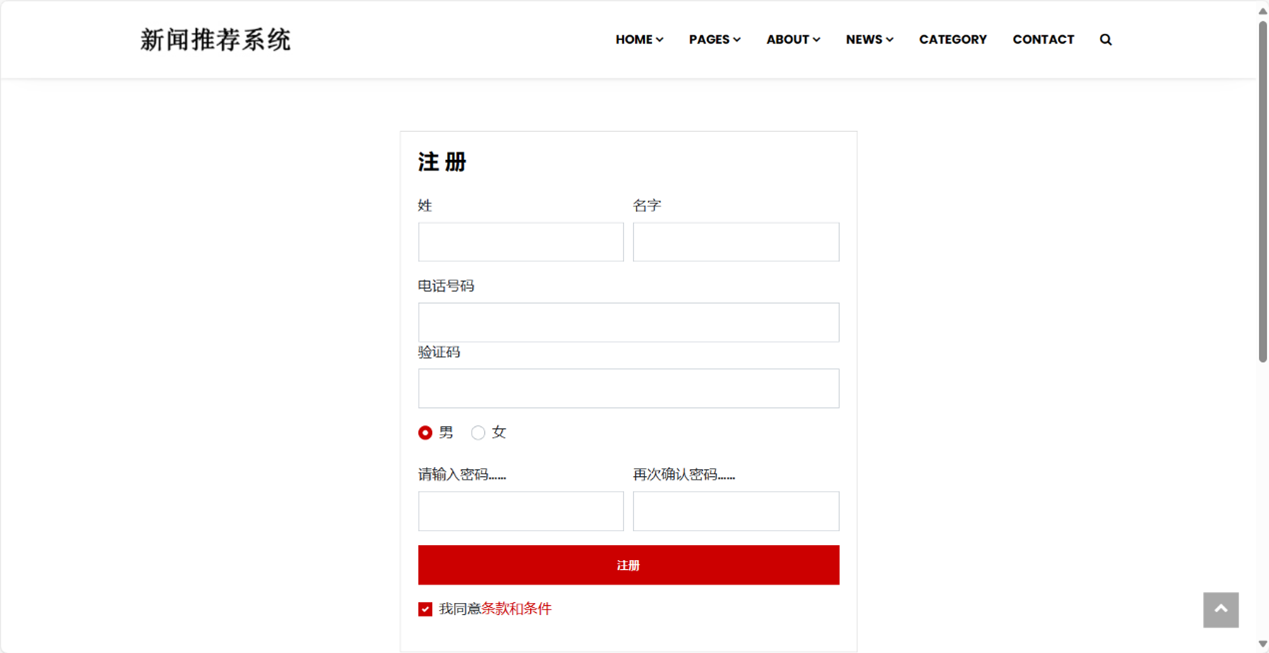
\includegraphics[width=0.75\textwidth]{用户注册页面}
		\caption{用户注册页面}
		\label{fig:circuit-diagcam}
	\end{figure}
	2.用户登录\par
	\begin{figure}[H]
		\centering
		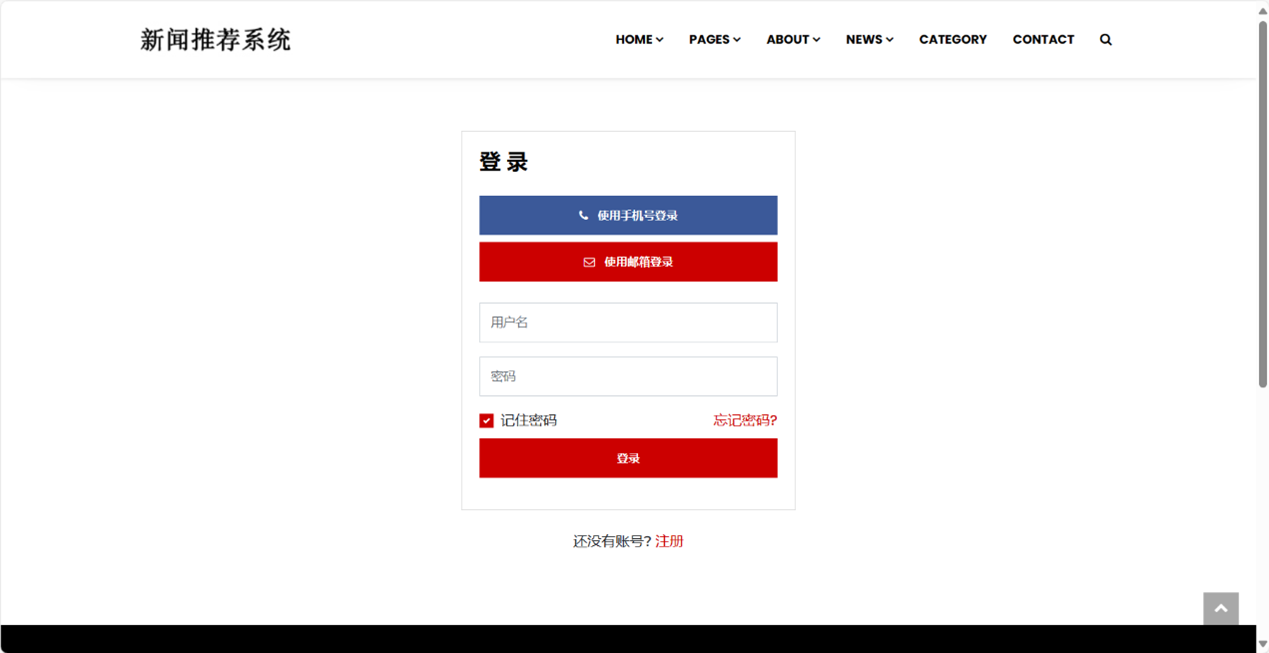
\includegraphics[width=0.75\textwidth]{用户登录页面}
		\caption{用户登录页面}
		\label{fig:circuit-diagcam}
	\end{figure}
	3.新闻内容浏览\par
	\begin{figure}[H]
		\centering
		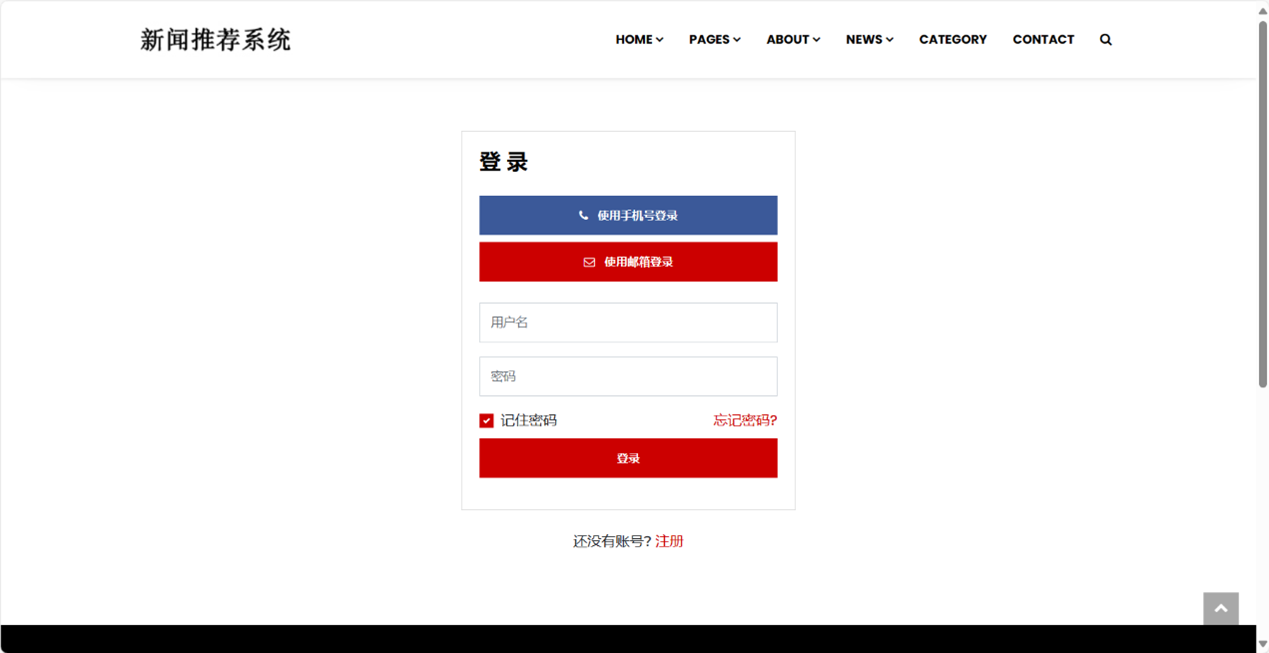
\includegraphics[width=0.75\textwidth]{用户登录页面}
		\caption{用户登录页面}
		\label{fig:circuit-diagcam}
	\end{figure}
	
	4.历史点击记录\par
	\begin{figure}[H]
		\centering
		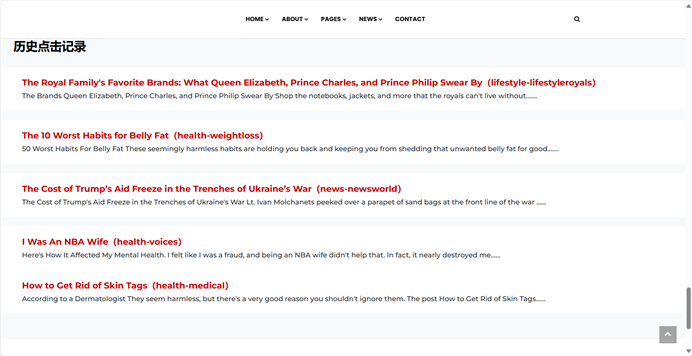
\includegraphics[width=0.75\textwidth]{历史点击记录页面}
		\caption{历史点击记录页面}
		\label{fig:circuit-diagcam}
	\end{figure}
	5.个性化推荐\par
	\begin{figure}[H]
		\centering
		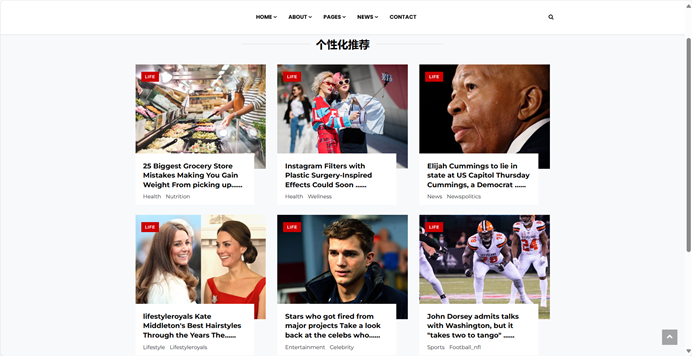
\includegraphics[width=0.75\textwidth]{个性化推荐页面}
		\caption{个性化推荐页面}
		\label{fig:circuit-diagcam}
	\end{figure}
	\subsubsection{ 兼容性测试与稳定性测试}
	$\bigstar$可执行测试:分别部署到不同性能的电脑上运行测试,均成功运行,网页反馈
	均在35ms到45ms左右,不存在延迟和卡顿现象,该系统对电脑的配置要求较低。\par
	$\bigstar$功能测试:所有功能均可正常运行使用,首页展示
	效果正常,查询功能正常,链接页面跳转正常。\par
	$\bigstar$兼容测试:在 Windows、Linux、Mac等操作系统可以正常访问。谷歌浏览器、
	火狐浏览器、QQ 浏览器、360 浏览器等运行均正常。Windows操作系统的python版
	本为3.6以上、tensorflow1.15.4 版本环境可以正常运行平台。\par
	$\bigstar$安全测试:本项目采取的是 https 协议,安全性和可靠性比较高,jupyter 环境
	提供了三种安全级服务配置,可以按照实际的需求提升安全等级。\par
	\newpage
	\section{商业模式构建与经营管理}
	\subsection{市场竞争分析( 按照SWOT分析写,画一个图)}
	\subsection{投资回报分析}
	\subsection{盈利方式}
	\subsubsection{ 提供整套低耦合工业界解决方案}
	\subsubsection{ 提供整套成熟软件系统}
	\subsection{财务管理}( 引入COCOMOS)模型
	\subsection{营销战略}(前中后期的营销模式+六位一体策略)
	\newpage
	%参考文献
	\begin{thebibliography}{9}%宽度9
		[1]陈昌凤,袁雨晴.智能新闻业:生成式人工智能成为基础设施[J].内蒙古社会科学,2024,45(01):40-48.DOI:10.14137/j.cnki.issn1003-5281.2024.01.006.
	\end{thebibliography}
\end{document}
